\section{Introduction}

Natural language processing (NLP) tasks such as sentiment analysis \cite{maas-etal-2011-learning, Zhang-etal-15-cnn-sentiment} and spam detection are modeled as classification tasks, where instances are independently labeled.
Tasks such as part-of-speech tagging \cite{CoNLL2017-shared-UD} and named entity recognition \cite{CoNLL-2003-NER} are examples of structured classification tasks, where instance classification is decomposed into a sequence of per-token contextualized labels.
We can similarly cast neural machine translation (NMT), an example of a natural language generation (NLG) task, as a form of structured classification, where an instance label (a translation) is generated as a sequence of contextualized labels, here by an autoregressor (see Section \ref{sec:classifier-nlg}).

Since the parameters of modern machine learning (ML) classification models are estimated from training data, whatever biases exist in the training data will affect model performance.
Among those biases, \textit{class imbalance} is a topic of our interest.
Class imbalance is said to exist when one or more classes are not of approximately equal frequency in data.
%\change{this is good earlier in the intro in place of too much variable introduction}
The effect of class imbalance has been extensively studied in several domains where classifiers are used (see Section \ref{sec:rel-class-imb}).
With neural networks, the imbalanced learning problem is mostly targeted to computer vision tasks; NLP tasks are under-explored \cite{Johnson2019SurveyImbalance}. % However neural networks are being used for many domains including NLP.

Word types in natural language models resemble a Zipfian distribution, i.e. in any natural language corpus, we observe that a type's rank is roughly inversely proportional to its frequency. Thus, a few types are extremely frequent, while most of the rest lie on the long tail of infrequency.
Zipfian distributions cause two problems in classifier-based NLG systems:
\begin{enumerate}
    \itemsep0em
    \item \textbf{Unseen Vocabulary:}
    %\jon{i really don't know what this means. Open vocabulary? Not really a zipfian thing. since you only stick with class 2 why bother fighting this fight?}\tg{Yes, Open vocabulary. This is needed for emphasising why BPE is needed and that we are stuck with it. A linguist might argue why not use unsupervised morphology instead of BPE, we can say morphology segmentation does not close the tail, but BPE does which is what we need}
    Any hidden data set may contain types not seen in the finite set used for training. A sequence drawn from a Zipfian distribution is likely to have a large number of rare types, and these are likely to have not been seen in training.
    \item \textbf{Imbalanced Classes:} There are a few extremely frequent types and many infrequent types, causing an extreme imbalance.
    Such an imbalance, in other domains where classifiers are used, has been known to cause undesired biases and severe performance degradation \cite{Johnson2019SurveyImbalance}. %\jon{citations here or you will be attacked for this line}
\end{enumerate}

%A few solutions exist to address the infinite vocabulary problem and are described in Section~\ref{sec:rel-finite-vocab}. Most notably, the use of byte pair encoding (BPE) subwords \cite{sennrich-etal-2016-bpe} addresses infinite vocabulary by using only a finite set of subwords.
The use of \textit{subwords}, that is, decomposition of word types into pieces
% more likely to have been seen in training
, such as the widely used Byte Pair Encoding (BPE) \cite{sennrich-etal-2016-bpe} addresses the open-ended vocabulary problem by ultimately allowing a word to be represented as a sequence of characters if necessary.
BPE has a single hyperparameter named \textit{merge operations} that governs the vocabulary size.
The effect of this hyperparameter is not well understood.
In practice, it is either chosen arbitrarily or via trial-and-error \cite{DBLP:journals/corr/abs-1810-08641}.

Regarding the problem of imbalanced classes, \newcite{steedman-2008-last} states that ``the machine learning techniques that we rely on are actually very bad at inducing systems for which the crucial information is in rare events.''
%and foresaw that \textit{``One day, either because of the demise of Moore’s law, or simply because we have done all the easy stuff, the Long Tail will comeback to haunt us"}.
However, to the best of our knowledge, this problem has not yet been directly addressed in the NLG setting.


Model-based metrics for evaluating MT such as BLEURT \cite{sellam-etal-2020-bleurt}, ESIM \cite{mathur-etal-2019-ESIM}, and YiSi \cite{lo-2019-yisi} have recently attracted attention due to their superior correlation with human judgments \cite{WMT19-metrics-proceedings}. However, \bleu~\cite{papineni-etal-2002-bleu} remains  the most widely used corpus-level MT metric. It correlates reasonably well with human judgments, and moreover is easy to understand and cheap to calculate, requiring only reference translations in the target language. By contrast, model-based metrics require tuning on thousands of examples of human evaluation for every new target language or domain \cite{sellam-etal-2020-bleurt}.
Model-based metric scores are also opaque and can hide undesirable biases, as can be seen in Table~\ref{tab:bleurt-bias}.


\begin{table}[ht]
    \centering
    %\footnotesize
    \begin{tabular}{l l l }
Reference:& \multicolumn{2}{l}{You must be a doctor.} \\
Hypothesis: & \multicolumn{2}{l}{$\rule{1cm}{0.15mm}$ must be a doctor.} \\
    % & You &	~0.990 \\
    & He	&-0.735 \\
    %& Alexandra & -0.888 \\
    %& Alexander & -0.975 \\
    & Joe & -0.975 \\
    & Sue & -1.043 \\
    & She	 &-1.100 \\\hline
Reference:& \multicolumn{2}{l}{It is the greatest country in the world.} \\
Hypothesis:& \multicolumn{2}{l}{$\rule{1cm}{0.15mm}$ is the greatest country in the world.} \\
    % & It	& ~0.957 \\
    & France &	-0.022 \\
    & America	& -0.060 \\
    & Russia &	-0.161 \\
    %& China  & -0.166 \\
    %& USA    & -0.168 \\
    %& India   &	-0.211 \\
    & Canada  & -0.309 
    \end{tabular}
    \caption{A demonstration of BLEURT's internal biases; model-free metrics like BLEU would consider each of the errors above to be equally wrong.}
    \label{tab:bleurt-bias}
\end{table}

The source of model-based metrics' (e.g. BLEURT) correlative superiority over model-free metrics (e.g. BLEU) appears to be the former's ability to focus evaluation on \textit{adequacy}, while the latter are overly focused on \textit{fluency}. BLEU and most other generation metrics consider each output \textit{token} equally. Since natural language is dominated by a few high-count types, an MT model that concentrates on getting its \textit{if}s, \textit{and}s and \textit{but}s right will benefit from BLEU in the long run more than one that gets its \textit{xylophone}s, \textit{peripatetic}s, and \textit{defenestrate}s right. Can we derive a metric with the discriminating power of BLEURT that does not share its bias or expense and is as interpretable as BLEU? 

As it turns out, the metric may already exist and be in common use. The areas concerned with classification such as information extraction have long used both \textit{micro averaging}, which treats each token equally, and \textit{macro averaging}, which instead treats each \textit{type} equally, when evaluating. The latter in particular is useful on imbalanced test sets to avoid results dominated by overly frequent types. In this work we take a classification-based approach to evaluating machine translation in order to obtain an easy-to-calculate metric that focuses on adequacy as much as BLEURT but does not have the expensive overhead, opacity, or bias of model-based methods. 

%In this work, we attempt to find answers to these questions: \textit{`What value of BPE vocabulary size is best for NMT?'}, and more crucially an explanation for \textit{`Why that value?'}.
%As we will see, the answers and explanations for those are an immediate consequence of a broader question, namely \textit{`What is the impact of Zipfian imbalance on classifier-based NLG?'}

The contributions of this paper are as follows:
We offer a simplified abstraction of NMT architectures by re-envisioning them as two high-level components: a multi-class \textit{classifier} and an \textit{autoregressor} (Section~\ref{sec:classifier-nlg}).
We describe some of the desired settings for the classifier (Section~\ref{sec:classifier-balance}) and autoregressor (Section~\ref{sec:ar-short-seq}) components.
In Section~\ref{sec:bpe}, we describe how vocabulary size choice relates to the desired settings for the two components.
Our experimental setup is described in Section~\ref{sec:exp-setup}, followed by an analysis of results in Section~\ref{sec:nmt_analysis} that offers an explanation with evidence for \textit{why} some vocabulary sizes are better than others.
Building upon our view of NMT as multi-class classifier, Section \ref{sec:mt-eval-as-cls} describes evaluation of NMT using standard classifier evaluation metrics such as precision, recall, and F-measure.
Section~\ref{sec:class-bias} uncovers the impact of class imbalance, particularly frequency based discrimination and how it affects precision and recall of classes.\footnote{In this work, `type' and `class' are used interchangeably.}
Section \ref{sec:justific-mt-eval} justifies macro-averaged F-measure as a legitimate MT evaluation metric.
%Section~\ref{sec:related-work} provides an overview of related work and Section~\ref{sec:conclusion} ends with a conclusion.

%%%%%%%%%%%%%%%%%%%%%%%%%%%%%%%%%%%%%%%%%%%%%%%%%%%%%%%%%%%%%%%%%%%%%%%%%%%%%%%%%%%%%%%%%%%%%%%
\section{Classifier based NLG}
\label{sec:classifier-nlg}

Machine translation is commonly defined as the task of transforming sequences from the form $x = x_1 x_2 x_3 ... x_m$ to $y = y_1 y_2 y_3 ... y_n$, where $x$ is in source language $X$ and $y$ is in target language $Y$.
%NMT accomplishes the translation objective using artificial neural networks.
There are many variations of NMT architectures (Section \ref{sec:rel-nmt-arch}), however, all share the common objective of maximizing ${ \prod_{t=1}^{n} P(y_t | y_{<t}, x_{1:m})}$ for pairs $(x_{1:m}, y_{1:n})$ sampled from a parallel dataset.
NMT architectures are commonly viewed as encoder-decoder networks.
We instead re-envision the NMT architecture as two higher level components: an autoregressor ($R$) and a token classifier ($C$), as shown in Figure~\ref{fig:nmt-architecture}.
\begin{figure}[ht]
    \centering
    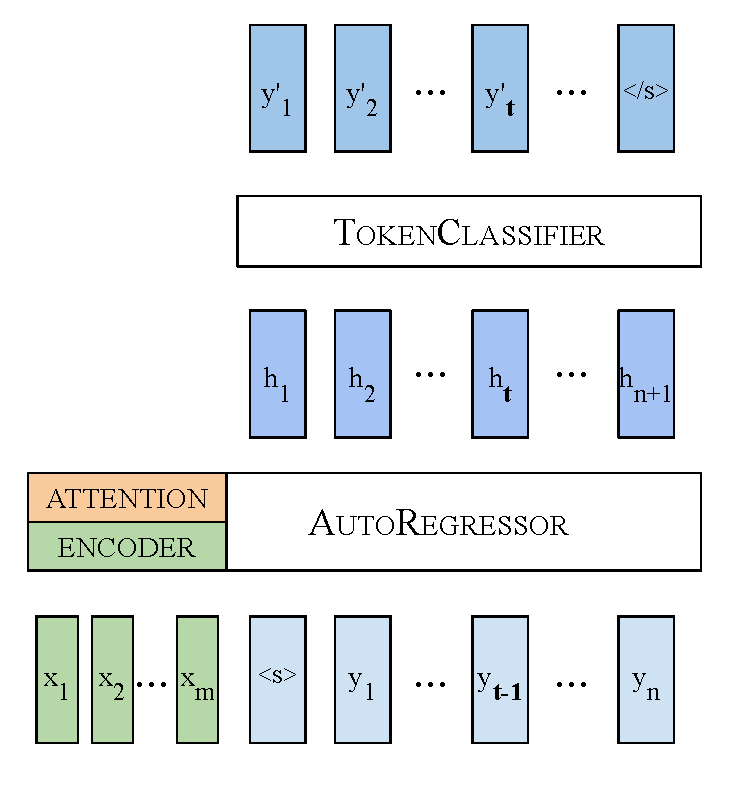
\includegraphics[height=0.35\textheight]{nmt-arch-classifier.pdf}
    \caption{The NMT model re-envisioned as a token classifier with an autoregressive feature extractor.}
    \label{fig:nmt-architecture}
%% to edit this, go to https://docs.google.com/drawings/d/1Ei9m3WanLJRvoegurFZpiSRQTz7p1Mmde25G0ZwnmAU/edit
\end{figure}

Autoregressor $R$, \cite{box2015time} being the most complex component of the NMT model,
%\footnote{The autoregressor is commonly associated with only the decoder of NMT. An ablation of Transformer NMT showed that the NMT functions even if there are no encoder layers, which leads to this simplification.}
has many implementations based on various neural network architectures: recurrent neural networks (RNN) such as long short-term memory (LSTM) and gated recurrent unit (GRU), convolutional neural networks (CNN), and Transformer (Section \ref{sec:rel-nmt-arch}).
At time step $t$, $R$ transforms the input context $y_{<t}, x_{1:m}$ into hidden state vector $h_t = R(y_{<t}, x_{1:m})$.

Classifier $C$ is the same across all architectures.
It maps $h_t$ to a distribution $P(y_j | h_t) \forall y_j \in V_Y$, where $V_Y$ is the vocabulary of $Y$.
%Intuitively, $C$ scores $h_t$ against an embedding of every class type, then transforms those arbitrarily ranged scores into a probability distribution using the \textsc{SoftMax} normalizer.
In machine learning, input to classifiers such as $C$ is generally described as features that are either hand-engineered or automatically extracted. % using neural networks.
In our high-level view of NMT architectures, $R$ is a neural network that serves as an automatic feature extractor for $C$.

%With this setup we analyze weaknesses of both $C$ and $R$ in the following sub sections.

\subsection{Balanced Classes for Token Classifier}
\label{sec:classifier-balance}

Untreated, class imbalance leads to bias based on class frequencies.
Specifically, classification learning algorithms focus on frequent classes while paying relatively less importance to infrequent classes.
Frequency-based bias leads to poor recall of infrequent classes \cite{Johnson2019SurveyImbalance}.
%In NMT, the poor precision of frequent classes lead to the over generation of frequent types which are usually \textit{stopwords} such as \textit{the} or words that contribute to fluency.
%The poor recall of infrequent class implies not generating infrequent words which are usually the content words.

When a model is used in a \textit{domain mismatch} scenario, i.e. where a test set's distribution does not match the training set's distribution, model performance generally degrades.
It is not surprising that frequency-biased classifiers show particular degradation in domain mismatch scenarios, as  types that were infrequent in the training distribution and were ignored by the learning algorithm may appear with high frequency in the new domain.
\newcite{koehn2017sixchallenges} showed empirical evidence of poor generalization of NMT to out-of-domain datasets.

In other classification tasks, where each instance is classified independently, methods such as up-sampling infrequent classes and down-sampling frequent classes are used.
In NMT, since classification is done within the context of sequences, it is possible to accomplish the objective of balancing by altering sequence lengths.
%We achieve this balance by altering the effective sequence length of the input, which
This can be done by choosing the level of subword segmentation \cite{sennrich-etal-2016-bpe}.
%Section \ref{sec:bpe} describes the effect of BPE subwords from the perspective of class balancing.

\textbf{Quantification of Zipfian Imbalance:}
We use two statistics to quantify the imbalance of a training distribution:

The first statistic relies on a measure of \textbf{Divergence} ($D$) from a balanced (uniform) distribution.
We use a simplified version of Earth Mover Distance, in which the total cost for moving a probability mass between any two classes  is the sum of the total mass moved.
Since any mass moved \textit{out of} one class is moved \textit{into} another, we divide the total per-class mass moves in half to avoid double counting.
Therefore, the imbalance measure $D$ on $K$ class distributions where $p_i$ is the observed probability of class $i$ in the training data is computed as:
$$D = \frac{1}{2} \sum_{i=1}^{K}| p_i - \frac{1}{K}|; \quad 0 \le D \le 1 $$

A lower value of $D$ is the desired setting for $C$, since the lower value results from a balanced class distribution.
When classes are balanced, they have approximately equal frequencies; biasing the classes based on their frequencies is unlikely.

The second statistic is \textbf{Frequency at 95th\% Class Rank (\textbf{$\mathcal{F}_{95\%}$})}, defined as the least frequency in the $95^{th}$ percentile of most frequent classes.
More generally, $\mathcal{F}_{\large{P\%}}$ is a simple way of quantifying the minimum number of training examples for at least the $P$th percentile of classes.
The bottom $(1-P)$ percentile of classes are overlooked to avoid the noise that is inherent in the real-world natural-language datasets.

A higher value for $\mathcal{F}_{95\%}$ is the desired setting for $C$, as a higher value indicates the presence of many training examples per class, and ML methods are known to perform better when there are many examples for each class.

\begin{comment}
\begin{figure}[ht]
    \centering
    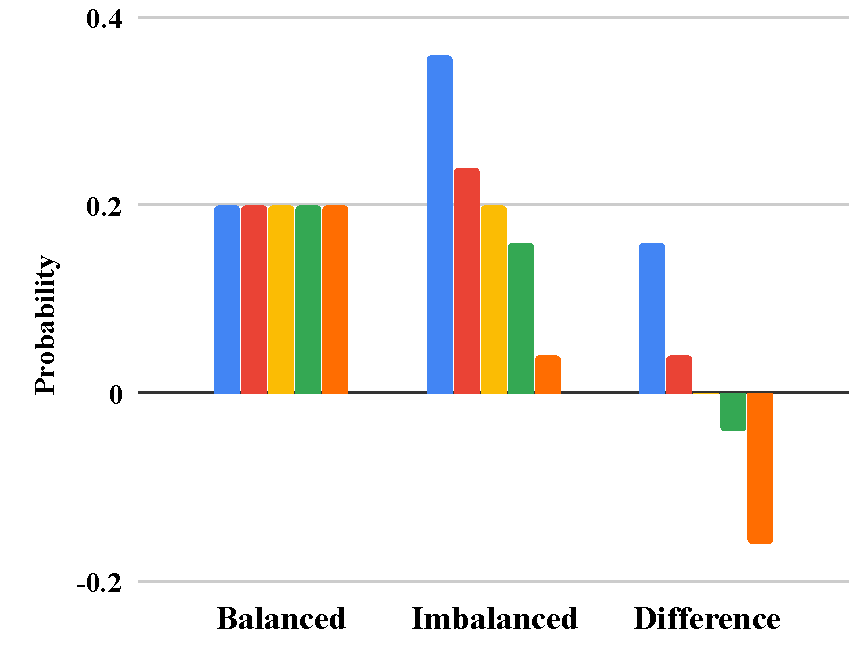
\includegraphics[width=0.8\linewidth]{imbalance-diff.pdf}
    \caption{An illustration of how class imbalance is quantified: Sum of the absolute differences between the observations and a balanced (uniform) distribution \change{this figure should be referenced somewhere in the main text. What is it you're trying to say in this figure? It is currently unclear what the bars represent, what the "difference" series is, etc.}}
\end{figure}
\end{comment}


\subsection{Shorter Sequences for Autoregressor}
\label{sec:ar-short-seq}

Every autoregressive model is an approximation; some may be better than others, but no model is perfect.
%Therefore, there is a non-zero probability of an error at each time step.
The total error accumulated grows in proportion to the length of the sequence.
These accumulated errors alter the prediction of subsequent tokens in the sequence.
Even though beam search attempts to mitigate this, it does not completely resolve it.
These challenges with respect to long sentences and beam size are examined by \newcite{koehn2017sixchallenges}.


We summarize sequence lengths using \textbf{Mean Sequence Length}, $\mu$,
computed trivially as the arithmetic mean of the lengths of \textit{target} language sequences after encoding them:
$\mu = \frac{1}{N} \sum_{i=1}^N |y^{(i)}|$
where $y^{(i)}$ is the $i$th sequence in the training corpus of $N$ sequences.
Since shorter sequences have relatively fewer places where an imperfectly approximated autoregressor model can make errors, a smaller $\mu$ is a desired setting for $R$.

%%%%%%%%%%%%%%%%%%%%%%%%%%%%%%%%%%%%%%%%%%%%%%%%%
\subsection{Choosing the Vocabulary Size Systematically}
\label{sec:bpe}

BPE~\cite{sennrich-etal-2016-bpe} is a greedy iterative algorithm often used to segment a vocabulary into useful \textit{subwords}.
The algorithm starts with characters as its initial vocabulary.
In each iteration, it greedily selects the most frequent type bigram in the training corpus, and replaces the sequence with a newly created compound type.
Once the subword vocabulary is learned, it can be applied to a corpus by greedily segmenting words with the longest available subword type. These operations have an effect on $D$, $\mathcal{F}_{95\%}$, and $\mu$.

\textbf{Effect of BPE on $\mu$}:
BPE expands rare words into two or more subwords, lengthening a sequence (and raising $\mu$) relative to simple white-space segmentation.
BPE merges frequent-character sequences into one subword piece, shortening a sequence (and lowering $\mu$) relative to character segmentation.
Hence, the sequence length of BPE segmentation lies in between the sequence lengths obtained by white-space and character-only segmentation methods \cite{morishita-etal-2018-improving}. % is more general that the words and characters are special cases that are attained at the two extremes . \change{what does the previous sentence mean??}
% Therefore, the BPE hyperparamter can be used to create sequences that are as long as character sequences (i.e larger $\mu$), or short as white-space segmented word sequences (i.e smaller $\mu$).
% Hence, BPE vocabulary size alter $\mu$.

\textbf{Effect of BPE on $\mathcal{F}_{95\%}$ and $D$}:
Whether BPE is viewed as a merging of frequent subwords into a relatively less frequent compound, or a splitting of rare words into relatively frequent subwords, BPE alters the class distribution by moving the probability mass of classes.
Hence, by altering the class distribution, BPE also alters both $\mathcal{F}_{95\%}$ and $D$. The BPE hyperparameter controls the amount of probability mass moved between subwords and compounds.

Figure~\ref{fig:BPE-imbalance} shows the relation between number of BPE merges (i.e. the BPE hyperparameter), and both $D$ and $\mu$.
When few BPE merge operations are performed, we observe the lowest value of $D$, which is a desired setting for $C$, but at the same point $\mu$ is large and undesired for $R$ (Section~\ref{sec:classifier-nlg}).
When a large number of BPE merges are performed, the effect is reversed, i.e. we observe that $D$ is large and unfavorable to $C$ while $\mu$ is small and favorable to $R$.
In the following sections we describe our experiments and analysis to locate the optimal number of BPE merges that achieves the right trade-off for both $C$ and $R$.
% Hence, BPE vocabulary size is \textit{not} arbitrary since it can be tuned to reduce $D$ while keeping $\mu$ short enough as well.

%For a comparison, word and character segmentation have no influence on $\mu$. However, the trim size of word and character vocabulary has an effect on class imbalance $D$ and Out-of-Vocabulary (OOV) tokens.% and is presented in Figures~\ref{fig:word-imbalance} and \ref{fig:char-imbalance}, respectively.
%The summary of word, character, and BPE with respect to $D$ and $\mu$ is presented in Table~\ref{tab:analysis-encoding}.

 \begin{figure}[ht]
  \centering
    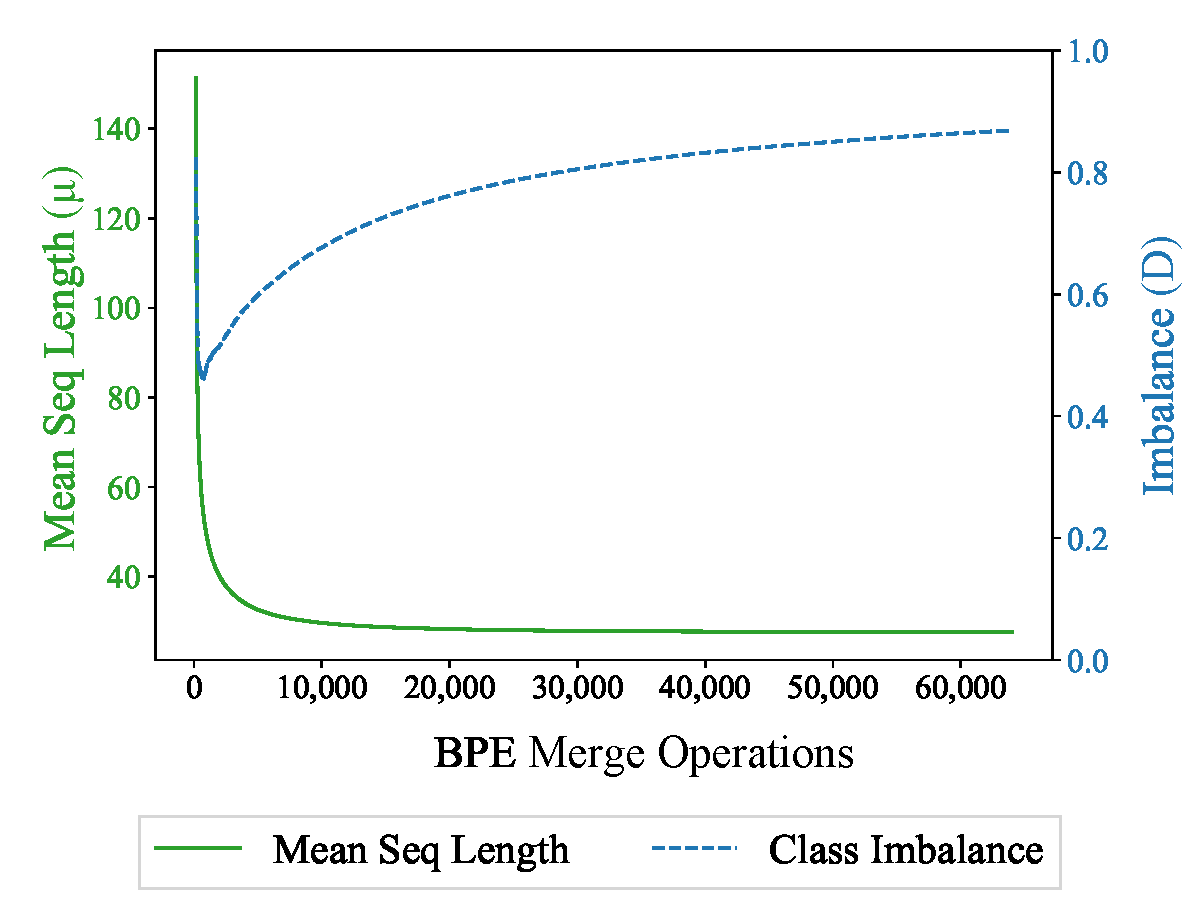
\includegraphics[width=0.75\linewidth]{bpe64k-deen-en.pdf}
    \caption{Effect of BPE merge operations on mean sequence length ($\mu$) and class imbalance ($D$).
    }
    \label{fig:BPE-imbalance}
\end{figure}


\section{Experimental Setup}
\label{sec:exp-setup}

Our NMT experiments use the base Transformer model \cite{vaswani2017attention} on four different target languages at various training data sizes, described in the following subsections.

\subsection{Datasets}
We use the following four language pairs for our analysis: English$\rightarrow$German, German$\rightarrow$English, English$\rightarrow$Hindi, and English$\rightarrow$Lithuanian.
To analyze the impact of different training data sizes, we randomly sub-select smaller training corpora for English$\leftrightarrow$German and English$\rightarrow$Hindi languages.
Statistics regarding the corpora used for validation, testing, and training are in Table~\ref{tab:datasets}.
The datasets for English$\leftrightarrow$German, and English$\rightarrow$Lithuanian are retrieved from the News Translation task of WMT2019~\cite{wmt19proceedings}.\footnote{\url{http://www.statmt.org/wmt19/translation-task.html}}
For English$\rightarrow$Hindi, we use the IIT Bombay Hindi-English parallel corpus v1.5~\cite{iitb-hien}.
English, German, and Lithuanian sentences are tokenized using \textsc{SacreMoses}.\footnote{\url{github.com/alvations/sacremoses}}
Hindi sentences are tokenized using \textsc{IndicNlpLibrary}.\footnote{\url{github.com/anoopkunchukuttan/indic_nlp_library}}
%The translations generated from NMT systems were consistently detokenized before scoring them using SacreBLEU \cite{post-2018-sacreBLEU}.
The training datasets are trivially cleaned: we exclude sentences with length in excess of five times the length of their parallel counterparts.
Since the vocabulary is a crucial part of this analysis, we exclude all sentence pairs containing URLs.

\begin{table*}[ht]
    \centering
    \footnotesize
\begin{tabular}{l l r r r l l}
  Languages & Training & Sentences & EN Toks & XX Toks & Validation & Test \\ \hline
\multirow{4}{1.5cm}{DE$\rightarrow$EN\\EN$\rightarrow$DE}
    & \multirow{4}{3.5cm}{Europarl v10 \\ \small{WMT13CommonCrawl} \\ \small{NewsCommentary v14}}
         & 30K  &  0.8M & 0.8M & \multirow{4}{*}{ {\small NewsTest18} }
            & \multirow{4}{*}{ \small{NewsTest19}} \\ \cdashline{3-5}
    &    & 0.5M  & 12.9M & 12.2M &  &  \\ \cdashline{3-5}
    &    & 1M    & 25.7M & 24.3M &  &  \\ \cdashline{3-5}
    &    & 4.5M  & 116M & 109.8M &  &  \\ \hdashline

\multirow{2}{*}{EN$\rightarrow$HI }
     & \multirow{2}{*}{ IITB Training }
         & 0.5M & 8M & 8.6M  & \multirow{2}{*}{ \small{IITB Dev} }
     & \multirow{2}{*}{ \small{IITB Test} }  \\\cdashline{3-5}
     &   & 1.3M & 21M & 22.5M   &   &  \\ \hdashline
EN$\rightarrow$LT & Europarl v10 & 0.6M & 17M & 13.4M  & \small{NewsDev19} & \small{NewsTest19} \\
\end{tabular}
    \caption{Training, validation, and testing datsets, along with sentence and token counts in training sets. We generally refer to dataset's sentence size in this work.}
    \label{tab:datasets}
\end{table*}

\subsection{Hyperparameters}
Our model is a 6 layer Transformer encoder-decoder that has 8 attention heads, 512 hidden vector units, and a feed forward intermediate size of 2048, with GELU activation.
We use label smoothing at 0.1, and a dropout rate of 0.1.
We use the Adam optimizer \cite{kingma2015adam} with a controlled learning rate that warms up for 16K steps followed by the decay rate recommended for training Transformer models~\cite{popel2018tfm-train-tips}.
To improve performance at different data sizes we set the mini-batch size to 6K tokens for the 30K-sentence datasets, 12K tokens for 0.5M-sentence datasets, and 24K for the remaining larger datasets~\cite{popel2018tfm-train-tips}.
All models are trained until no improvement in validation loss is observed, with a patience of 10 validations, each done at 1,000 update steps apart.
Our model is implemented using PyTorch and run on NVIDIA P100 and V100 GPUs.
To reduce padding tokens per batch, mini-batches are made of sentences having similar lengths \cite{vaswani2017attention}.
We trim longer sequences to a maximum of 512 tokens after BPE.
To decode, we average the last 10 checkpoints, and use a beam size of 4 with length penalty of 0.6, similar to \newcite{vaswani2017attention}.

Since the vocabulary size hyperparameter is the focus of this analysis, we use a range of vocabulary sizes that include character vocabulary and BPE operations that yield vocabulary sizes between 500 and 64K types.
A common practice, as seen in \newcite{vaswani2017attention}'s setup, is to jointly learn BPE for both source and target languages, which facilitates three-way weight sharing between the encoder's input, the decoder's input, and the output (i.e. classifier's class) embeddings \cite{press-wolf-2017-using}.
However, to facilitate fine-grained analysis of vocabulary sizes and their effect on class imbalance, our models separately learn source and target vocabularies; weight sharing between the encoder's and decoder's embeddings is thus not possible.
For the target language, however, we share weights between the decoder's input and the classifier's class embeddings.

\section{Results and Analysis}
%We use character and BPE subword encoding with various vocabulary sizes to analyze the effect of $D$ and $\mu$.
\label{sec:nmt_analysis}
\begin{figure}[ht]
\begin{subfigure}{0.70\linewidth}
    \centering
    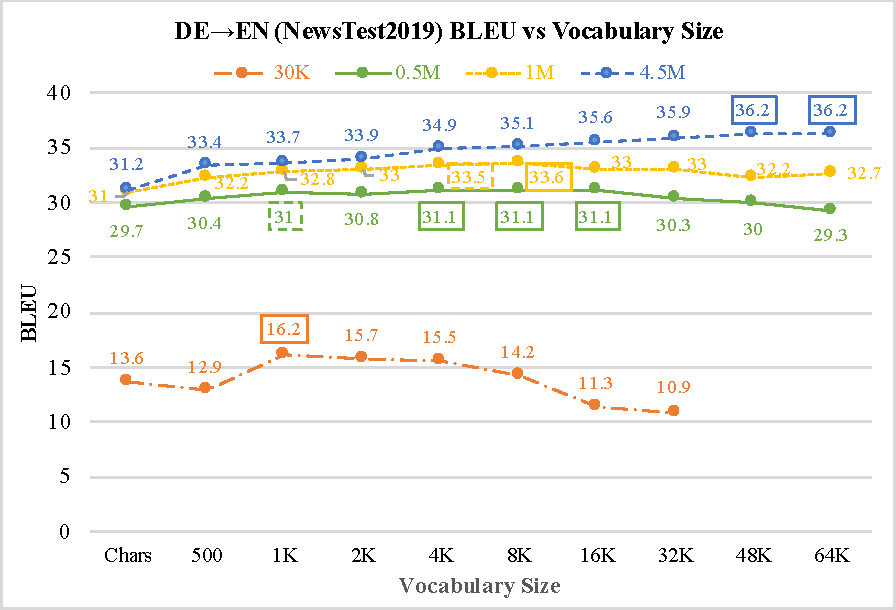
\includegraphics[width=\linewidth]{bleu-deen.pdf}
    \caption{DE$\rightarrow$EN BLEU on NewsTest2019}
    \label{fig:bleu-deen}
\end{subfigure}
\begin{subfigure}{0.70\linewidth}
    \centering
    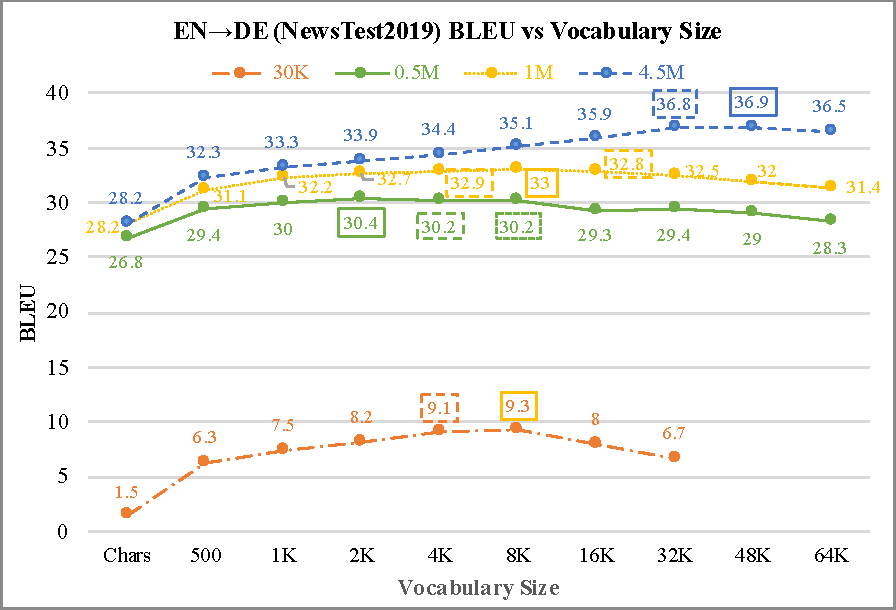
\includegraphics[width=\linewidth]{bleu-ende.pdf}
    \caption{EN$\rightarrow$DE BLEU on NewsTest2019}
    \label{fig:bleu-ende}
\end{subfigure}
\caption{EN$\leftrightarrow$DE NewsTest2019 BLEU as a function of vocabulary size at various training set sizes. 
Only the large dataset with 4.5M sentences has its best performance at a large vocabulary; all others peak at an 8K or smaller vocabulary size. Settings with the highest BLEU score are indicated by solid boundary and the ones within 0.2 BLEU to the highest BLEU are indicated by dashed boundary.}
\label{fig:bleu-ende-deen}
\end{figure}

\begin{figure}[ht]
    \centering
    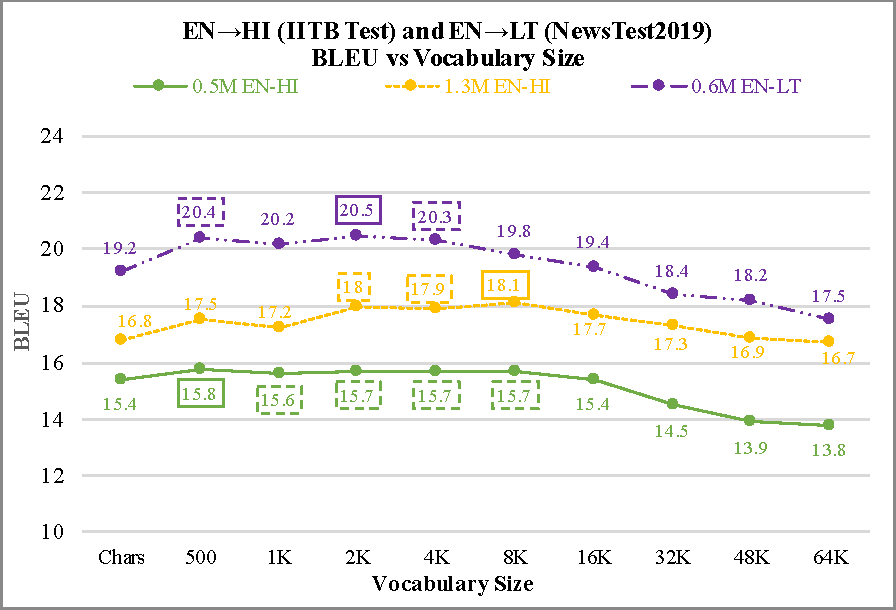
\includegraphics[width=0.70\linewidth]{bleu-enhi-enlt.pdf}
    \caption{BLEU on EN$\rightarrow$HI IITB Test and EN$\rightarrow$LT NewsTest2019 as a function of vocabulary size.  Settings with the highest BLEU score are indicated by solid boundary and the ones within 0.2 BLEU to the highest BLEU are indicated by dashed boundary.
    These language pairs observed the best BLEU scores in the range of 500 to 8K vocabulary size.   }
    \label{fig:bleu-enhilt}
\end{figure}


\begin{figure}[!ht]
\begin{subfigure}{\textwidth}
  \centering
  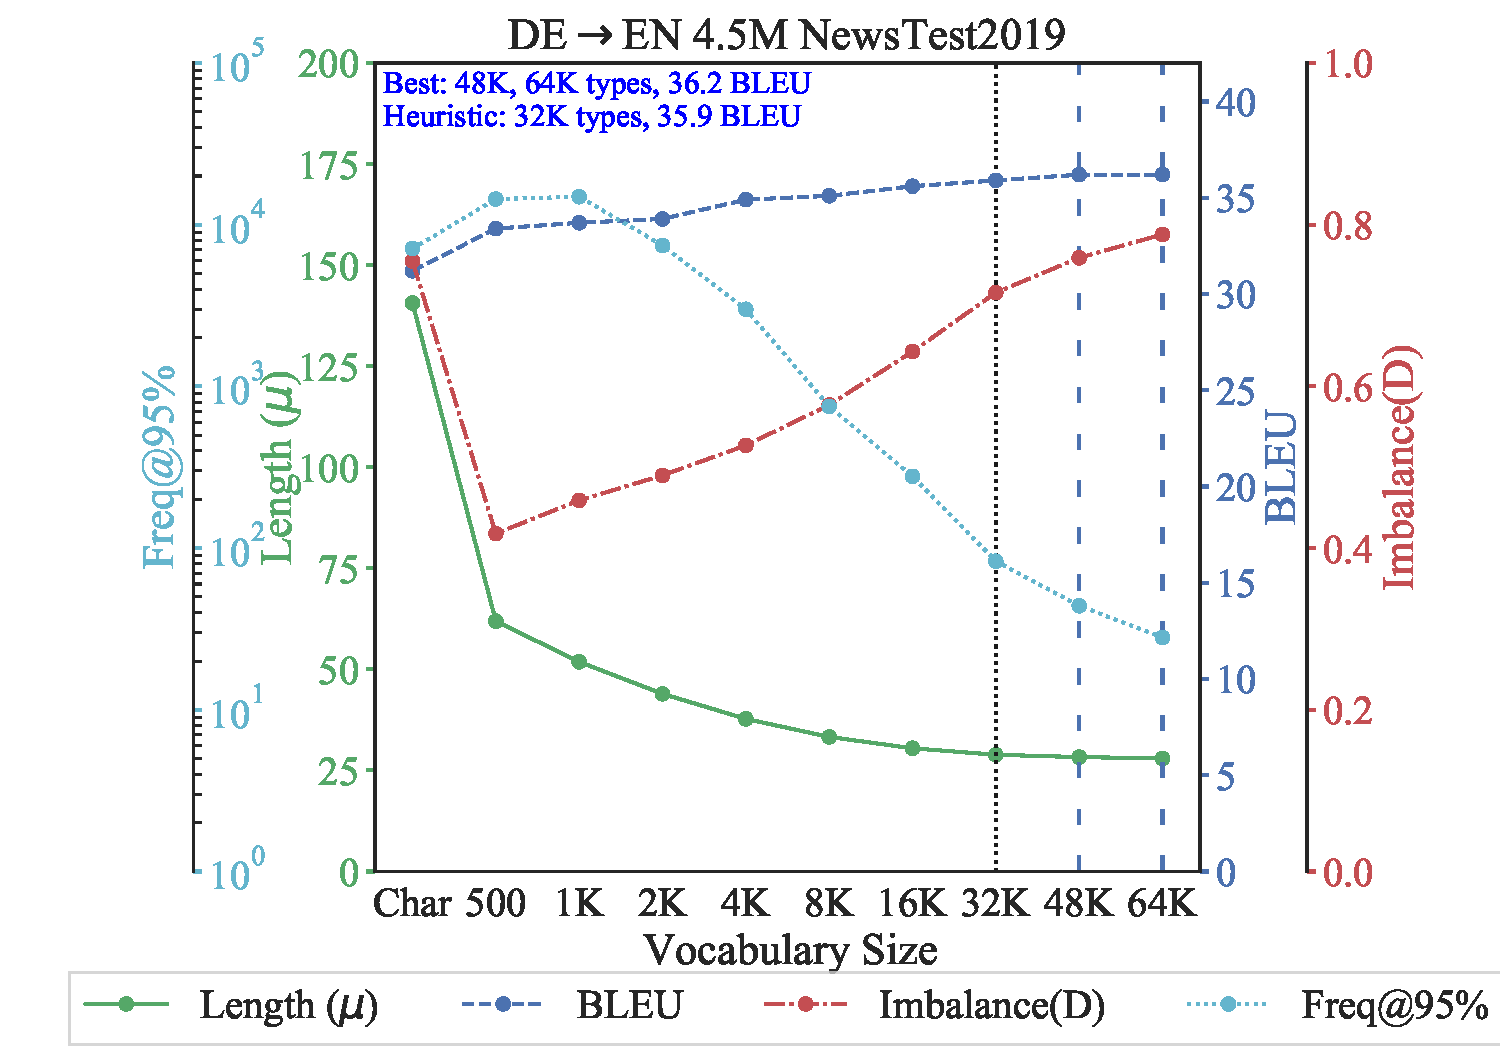
\includegraphics[width=0.7\linewidth,trim={1.4cm 0 0.2cm 16.45cm},clip]{4axv-test-deen-4.5m.pdf}
\end{subfigure}

\begin{subfigure}{.48\textwidth}
  \centering
  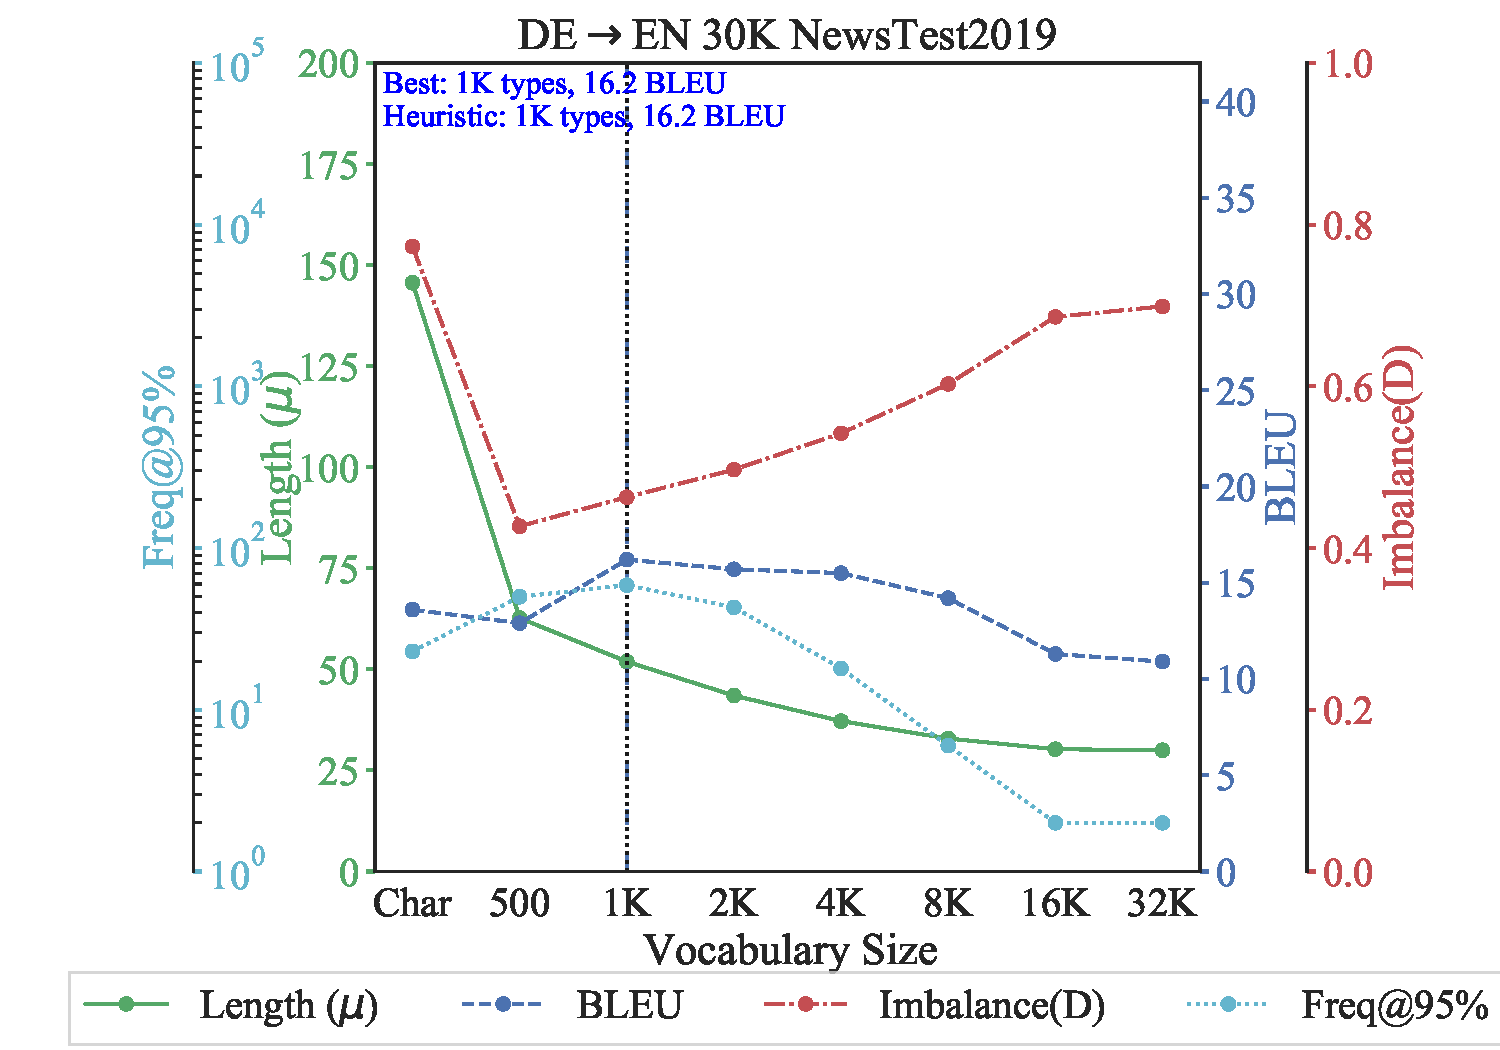
\includegraphics[width=0.96\linewidth,
  trim={2.4cm 1.32cm 4.1cm 0},clip]{4axv-test-deen-30k.pdf}
  %\caption{1a}
  %\label{fig:sfig1}
\end{subfigure}
\begin{subfigure}{.48\textwidth}
  \centering
  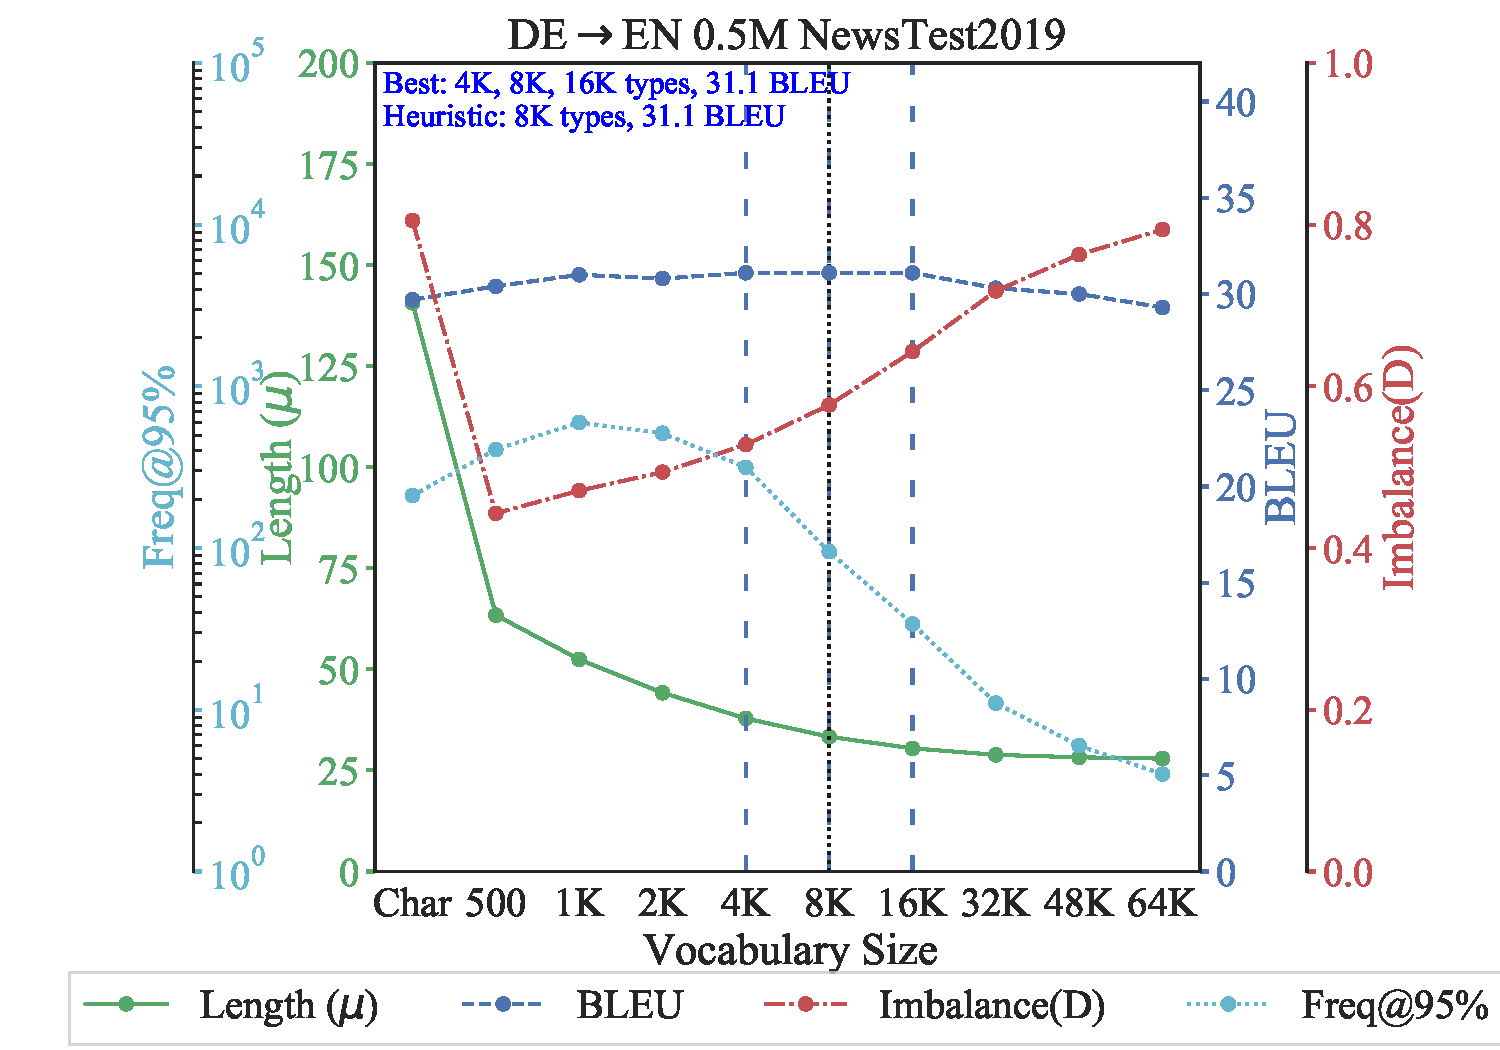
\includegraphics[width=0.96\linewidth,trim={5.1cm 1.32cm 1.4cm 0},clip]{4axv-test-deen-0.5m.pdf}
  %\caption{1c}
  %\label{fig:sfig2}
\end{subfigure}

\begin{subfigure}{.48\textwidth}
  \centering
  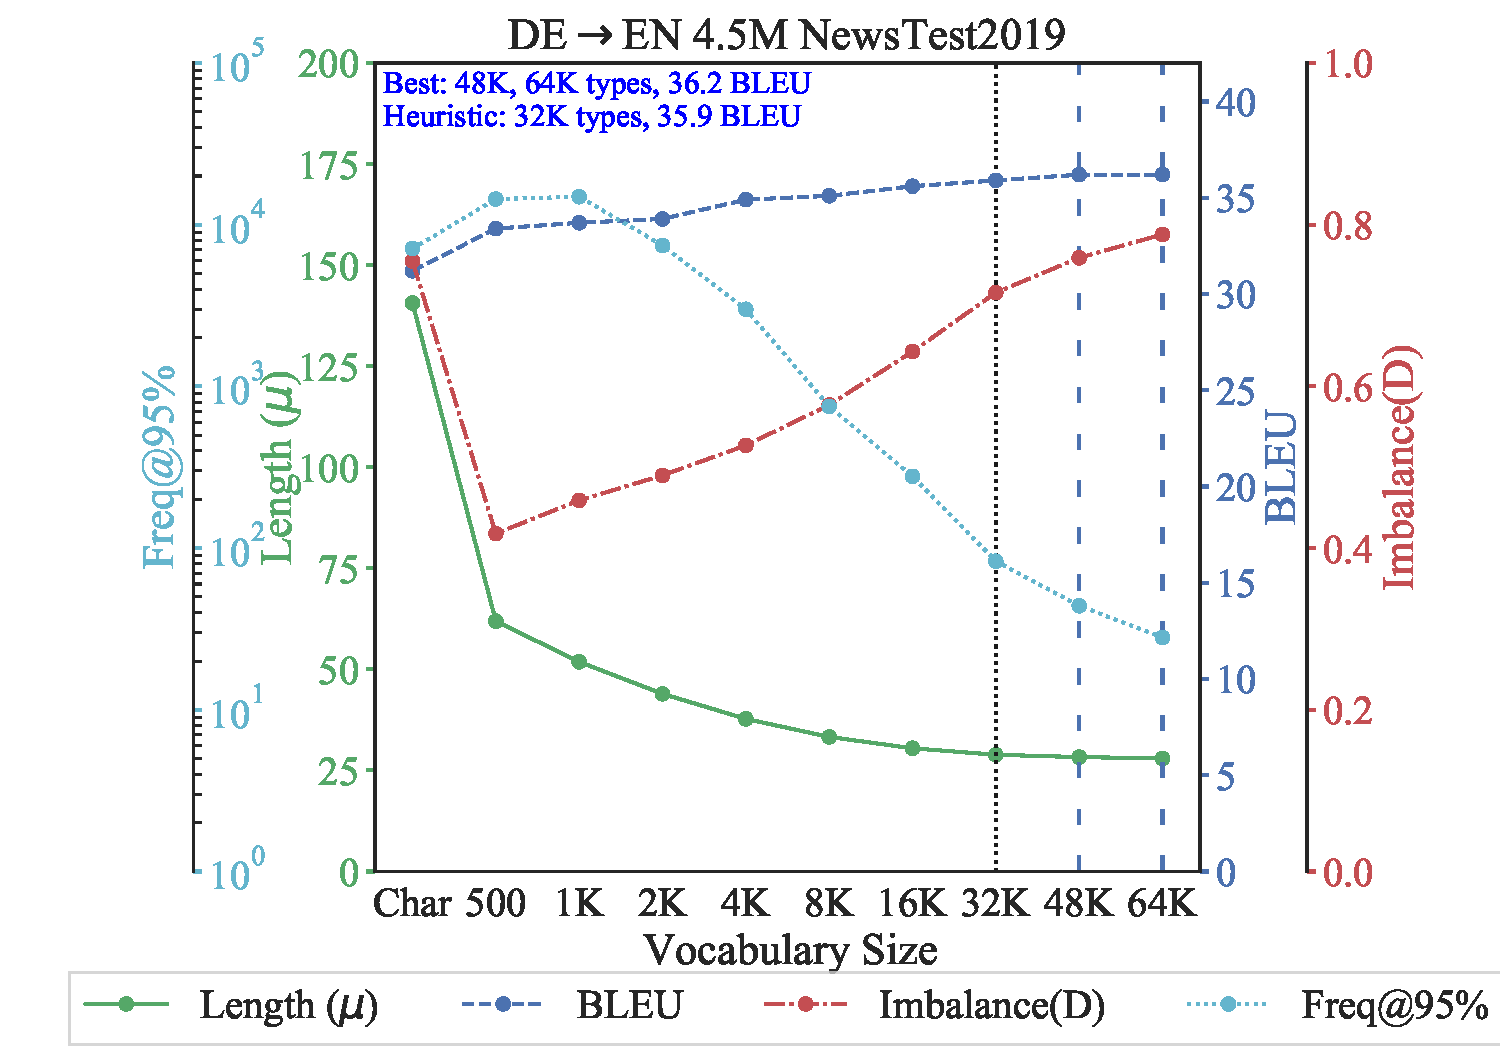
\includegraphics[width=0.96\linewidth,trim={2.4cm 1.32cm 4.1cm 0},clip]{4axv-test-deen-4.5m.pdf}
  %\caption{1c}
  %\label{fig:sfig2}
\end{subfigure}
\begin{subfigure}{.48\textwidth}
  \centering
  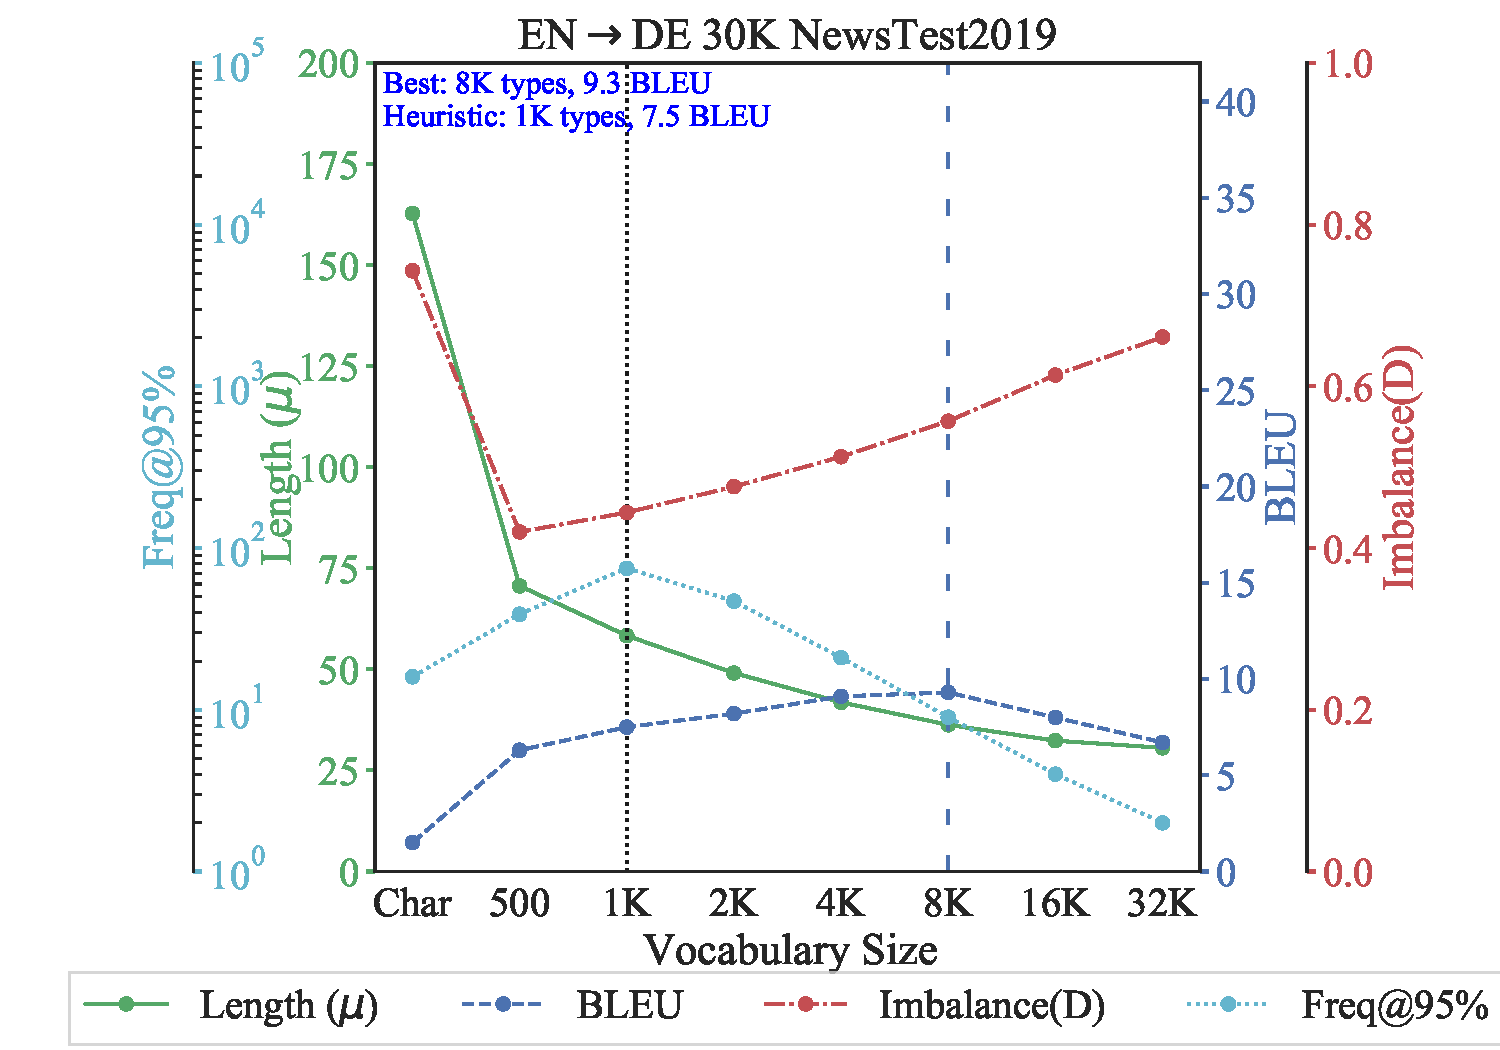
\includegraphics[width=0.96\linewidth,trim={5.1cm 1.32cm 1.4cm 0},clip]{4axv-test-ende-30k.pdf}
 % \caption{1a}
  %\label{fig:sfig1}
\end{subfigure}

\begin{subfigure}{.48\textwidth}
  \centering
  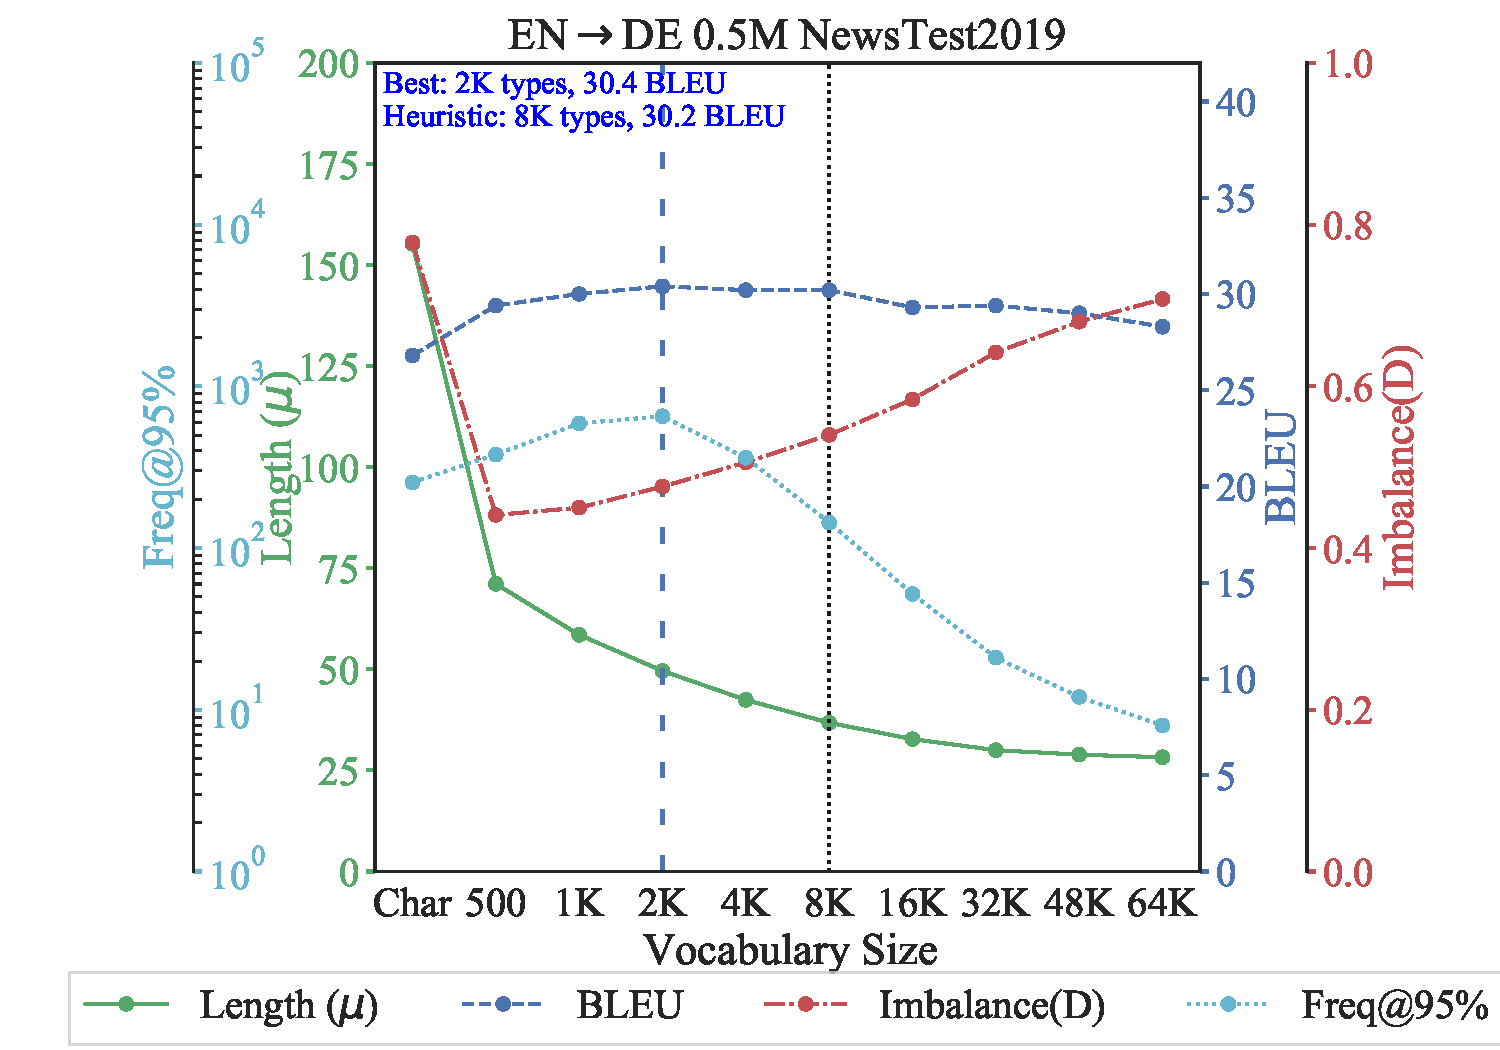
\includegraphics[width=0.96\linewidth,trim={2.4cm 1.32cm 4.1cm 0},clip]{4axv-test-ende-0.5m.pdf}
  %\caption{1c}
  %\label{fig:sfig2}
\end{subfigure}
\begin{subfigure}{.48\textwidth}
  \centering
  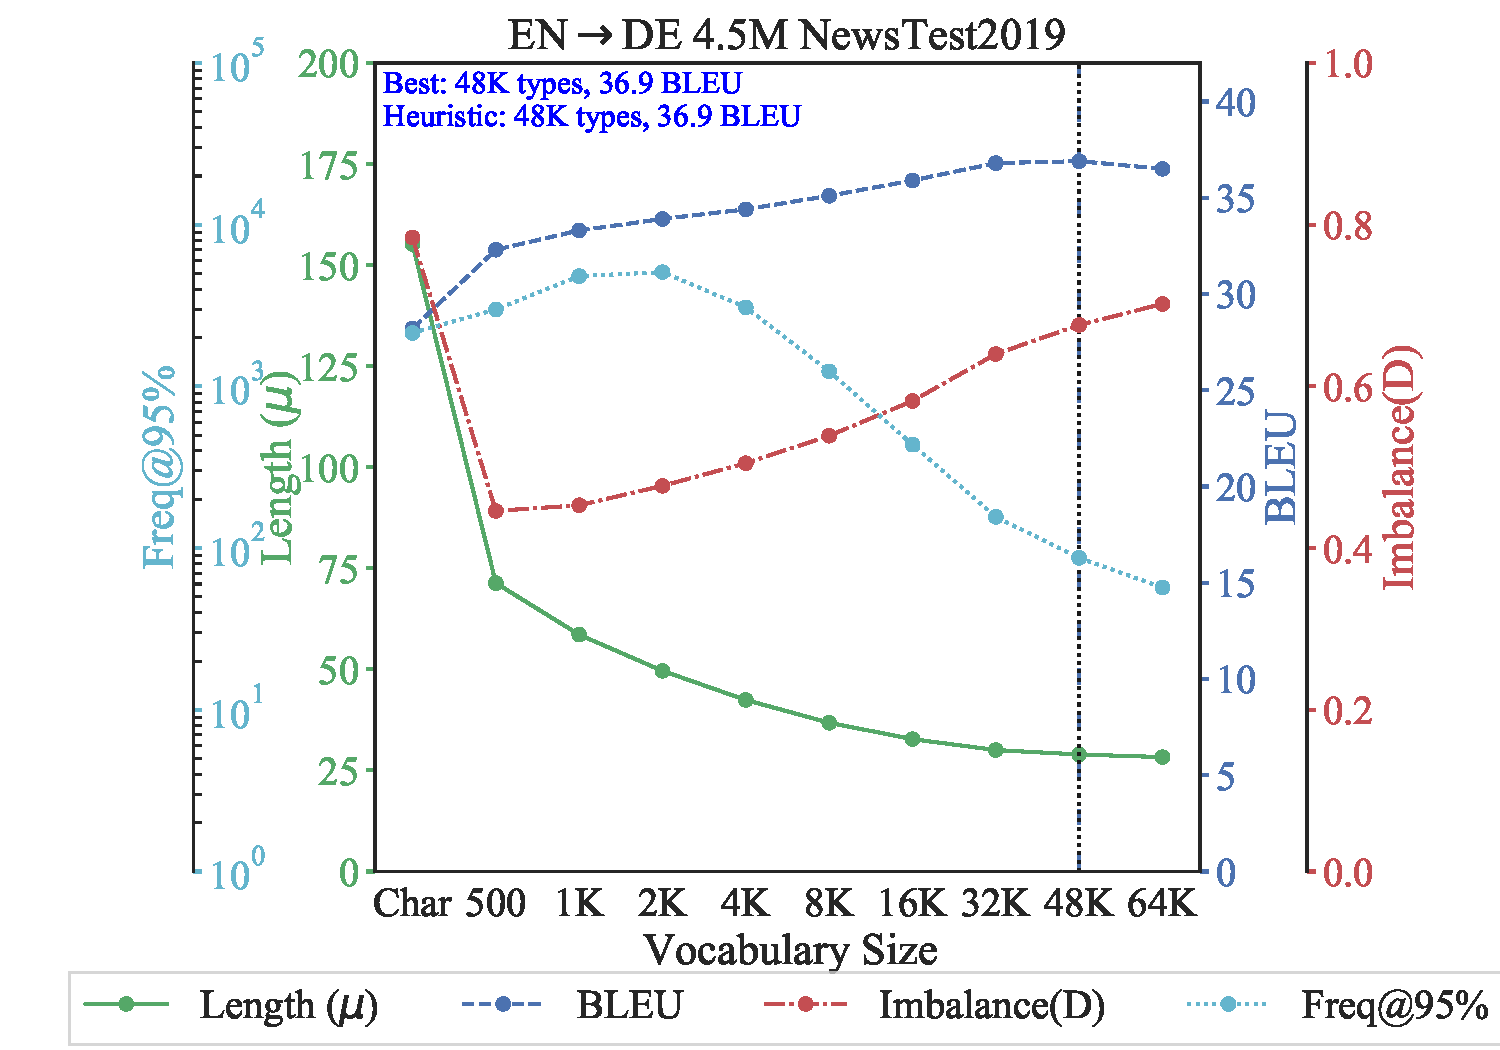
\includegraphics[width=0.96\linewidth,trim={5.1cm 1.32cm 1.4cm 0},clip]{4axv-test-ende-4.5m.pdf}
 % \caption{1c}
  %\label{fig:sfig2}
\end{subfigure}

\caption{Visualization of sequence length ($\mu$) (lower is better), class imbalance (D) (lower is better), frequency of $95^{th}$ percentile class ($\mathcal{F}_{95\%}$) (higher is better; plotted in logarithmic scale), and test set BLEU (higher is better) on all language pairs and training data sizes. % Visualizations on validation sets is provided in Appendix~\ref{sec:appendix}.
The vocabulary sizes that achieved highest BLEU are indicated with dashed vertical lines, and the vocabulary our heuristic selects is indicated by dotted vertical lines.}
\label{fig:mu-d-freq-bleu-part1}
\end{figure}

\begin{figure}[!ht]
\begin{subfigure}{\textwidth}
  \centering
  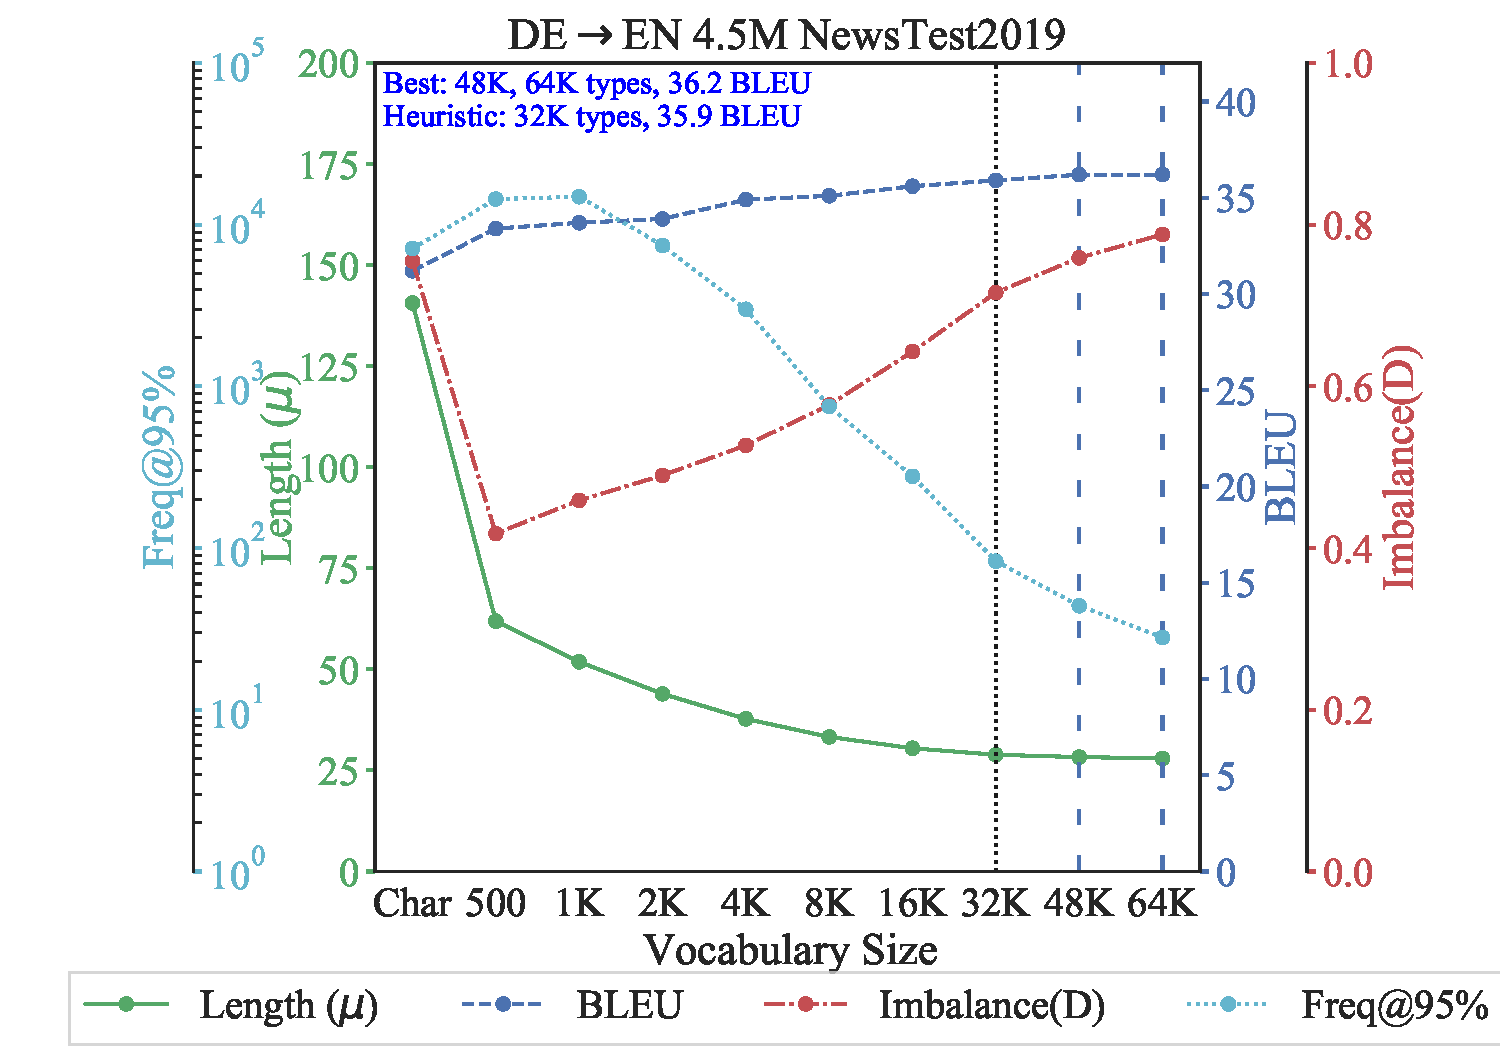
\includegraphics[width=0.7\linewidth,trim={1.4cm 0 0.2cm 16.45cm},clip]{4axv-test-deen-4.5m.pdf}
\end{subfigure}

\begin{subfigure}{0.48\linewidth}
  \centering
  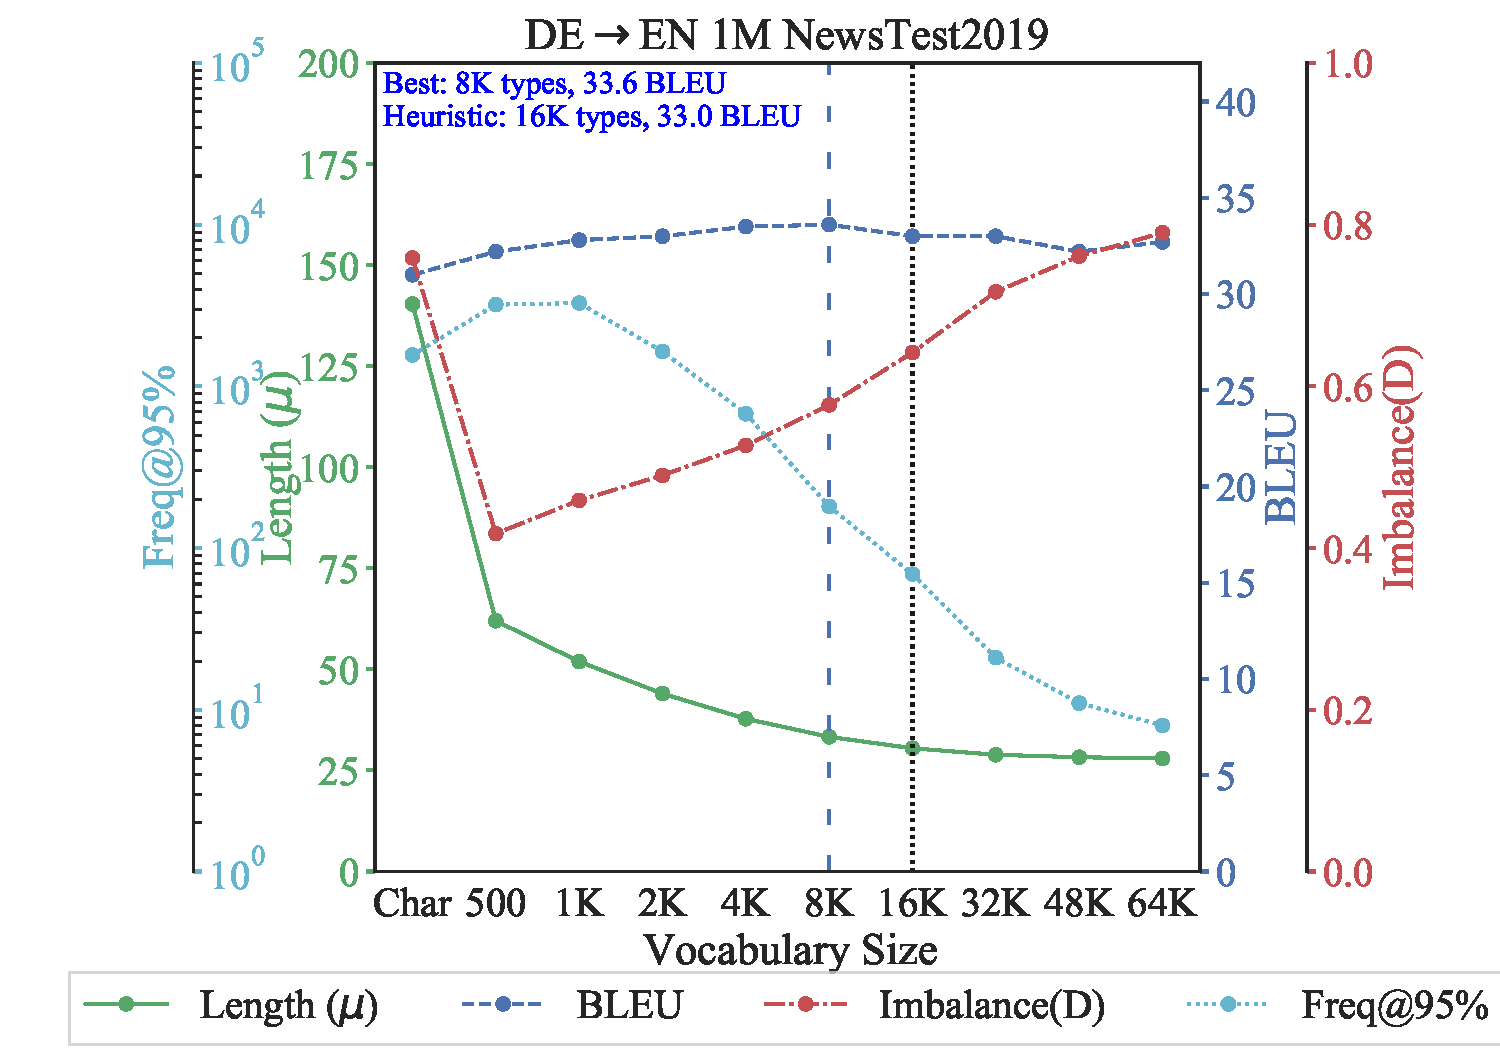
\includegraphics[width=0.96\linewidth,trim={2.4cm 1.32cm 4.1cm 0},clip]{4axv-test-deen-1m.pdf}
\end{subfigure}
\begin{subfigure}{0.48\linewidth}
  \centering
  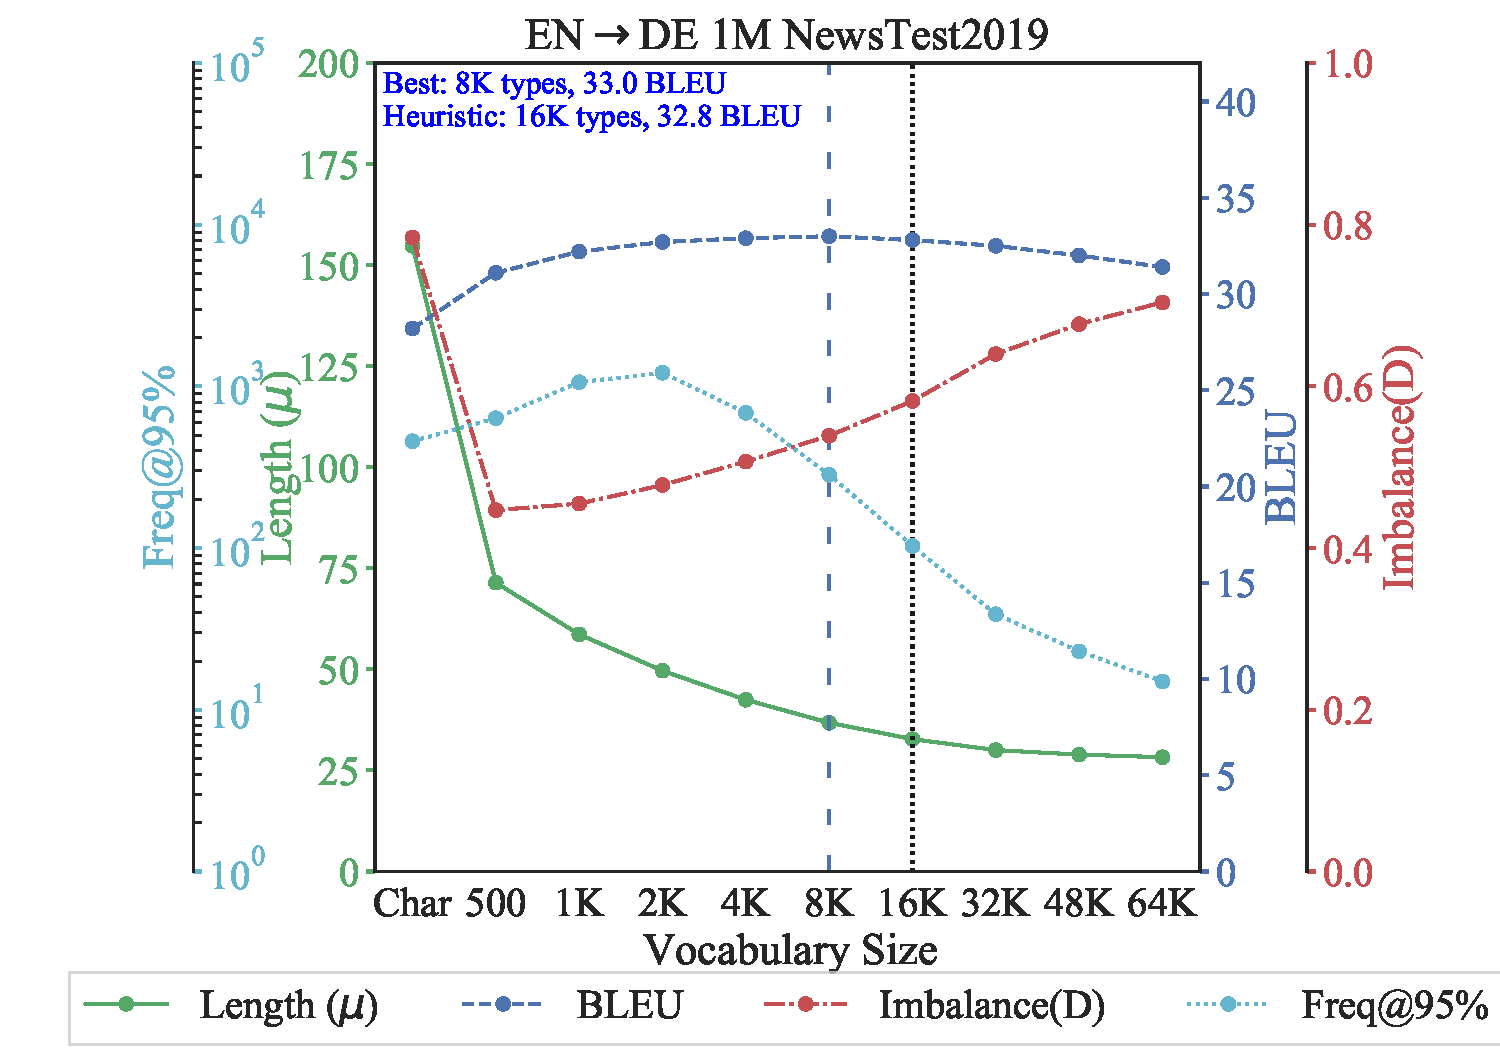
\includegraphics[width=0.96\linewidth,trim={5.1cm 1.32cm 1.4cm 0},clip]{4axv-test-ende-1m.pdf}
  %\caption{1c}
  %\label{fig:sfig2}
\end{subfigure}

\begin{subfigure}{.48\textwidth}
  \centering
  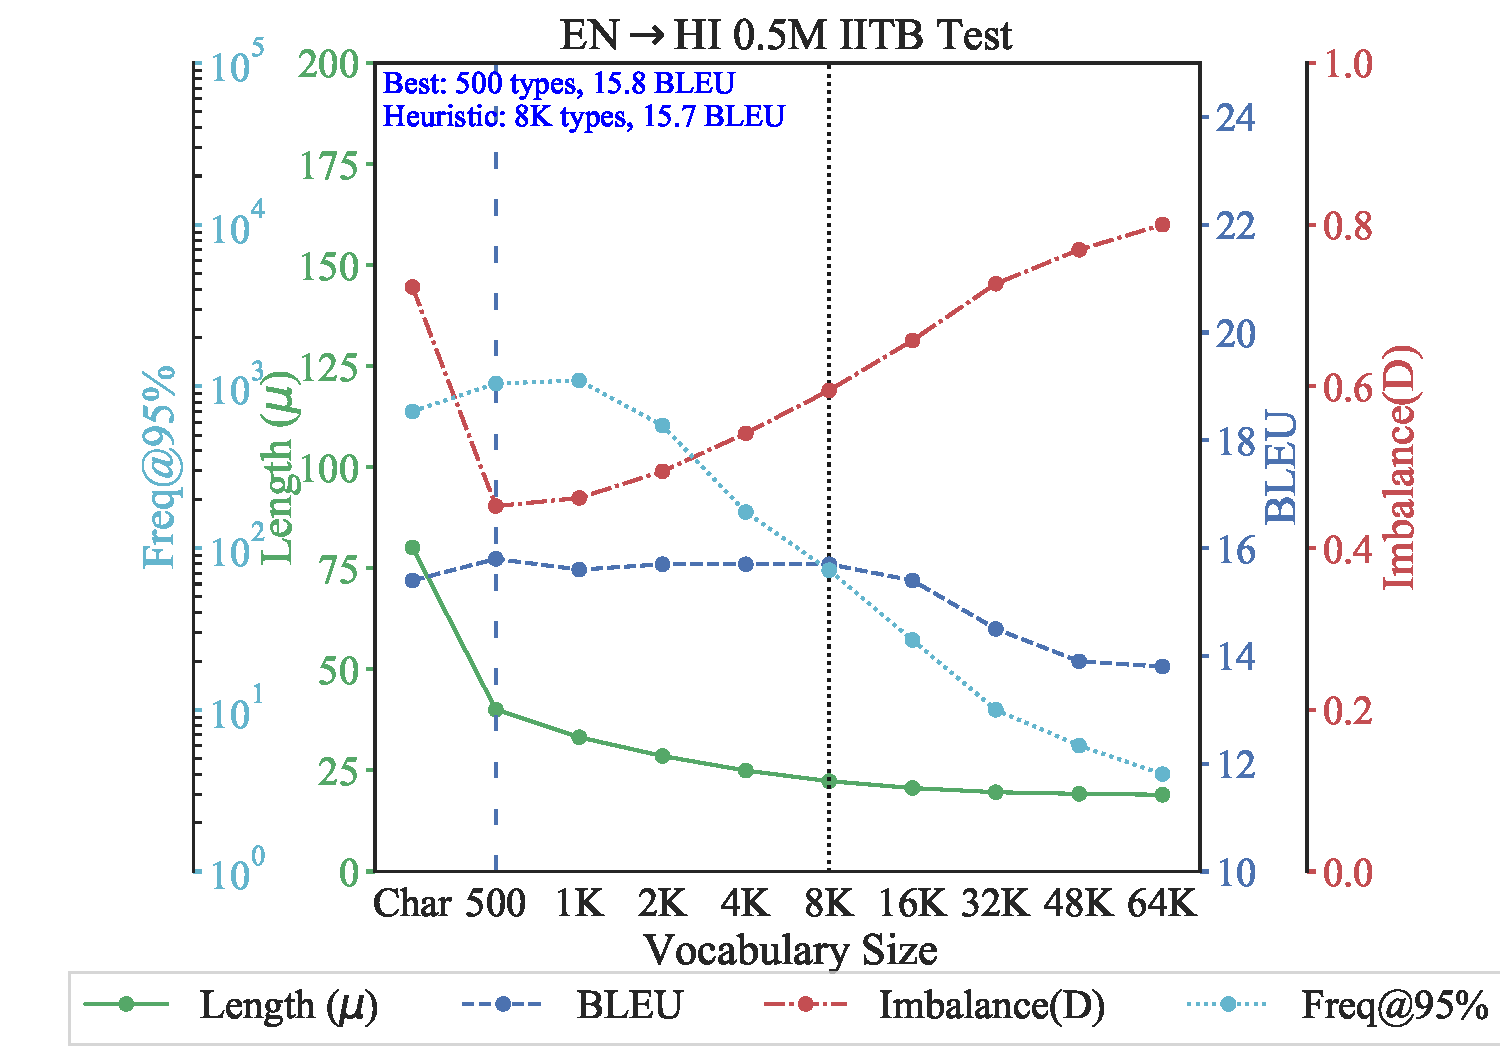
\includegraphics[width=0.96\linewidth,trim={2.4cm 1.32cm 4.1cm 0},clip]{4axv-test-enhi-0.5m.pdf}
 % \caption{1a}
  %\label{fig:sfig1}
\end{subfigure}
\begin{subfigure}{.48\textwidth}
  \centering
  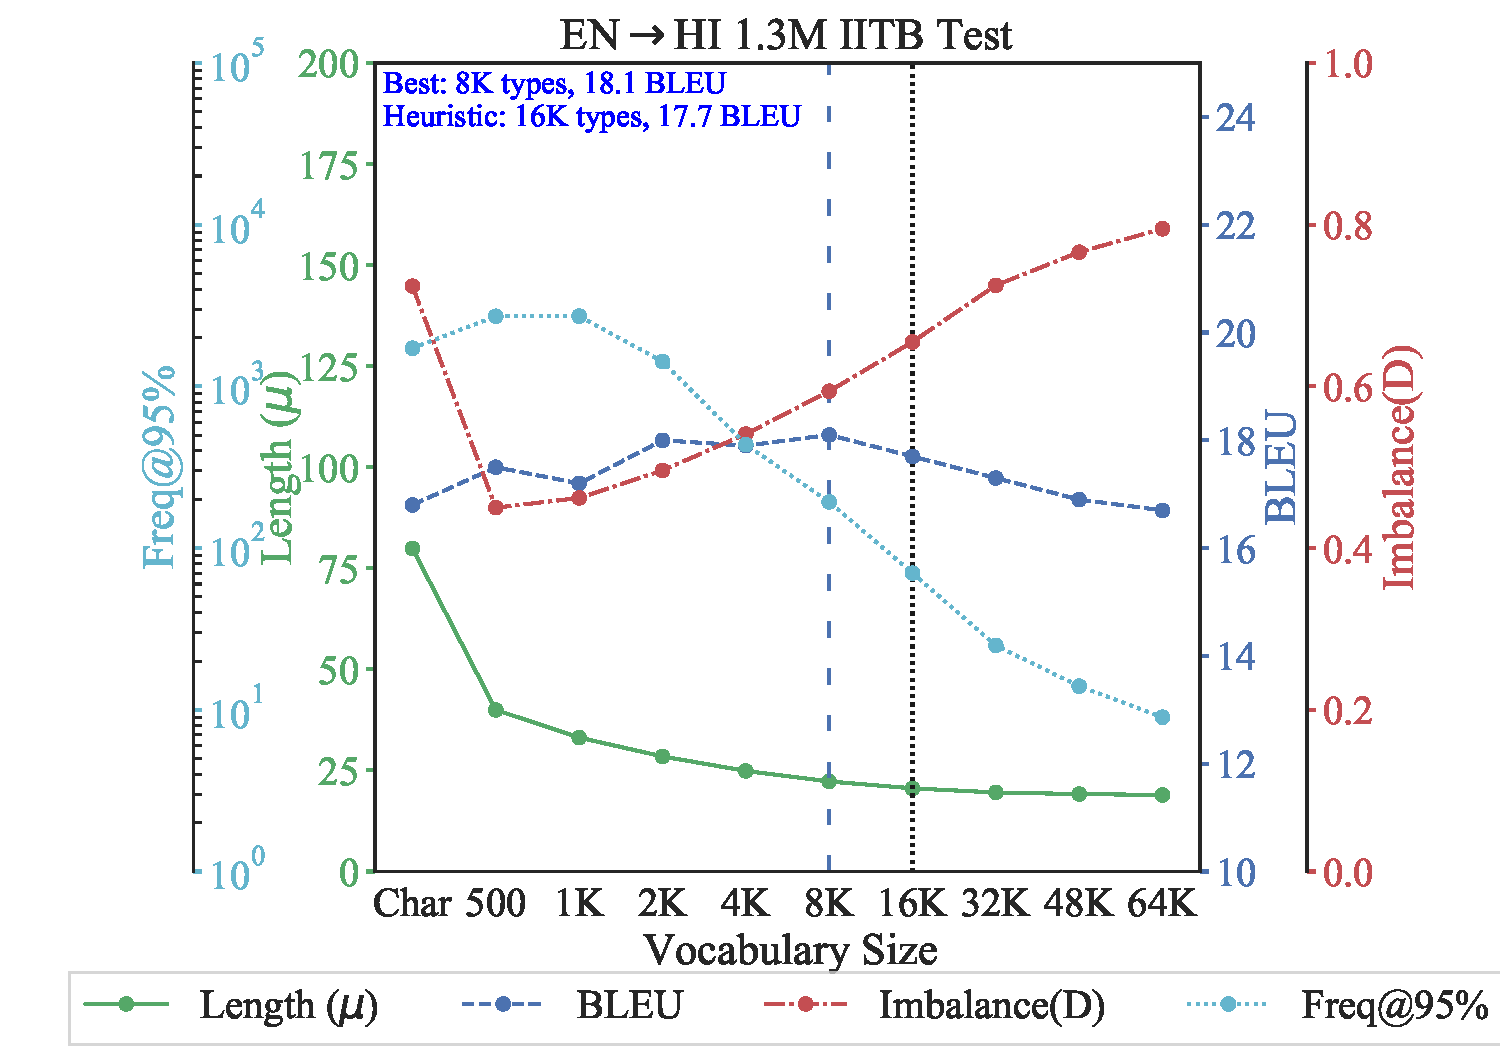
\includegraphics[width=0.96\linewidth,trim={5.1cm 1.32cm 1.4cm 0},clip]{4axv-test-enhi-1.3m.pdf}
  %\caption{1c}
  %\label{fig:sfig2}
\end{subfigure}


\begin{subfigure}{.55\textwidth}
  \centering
  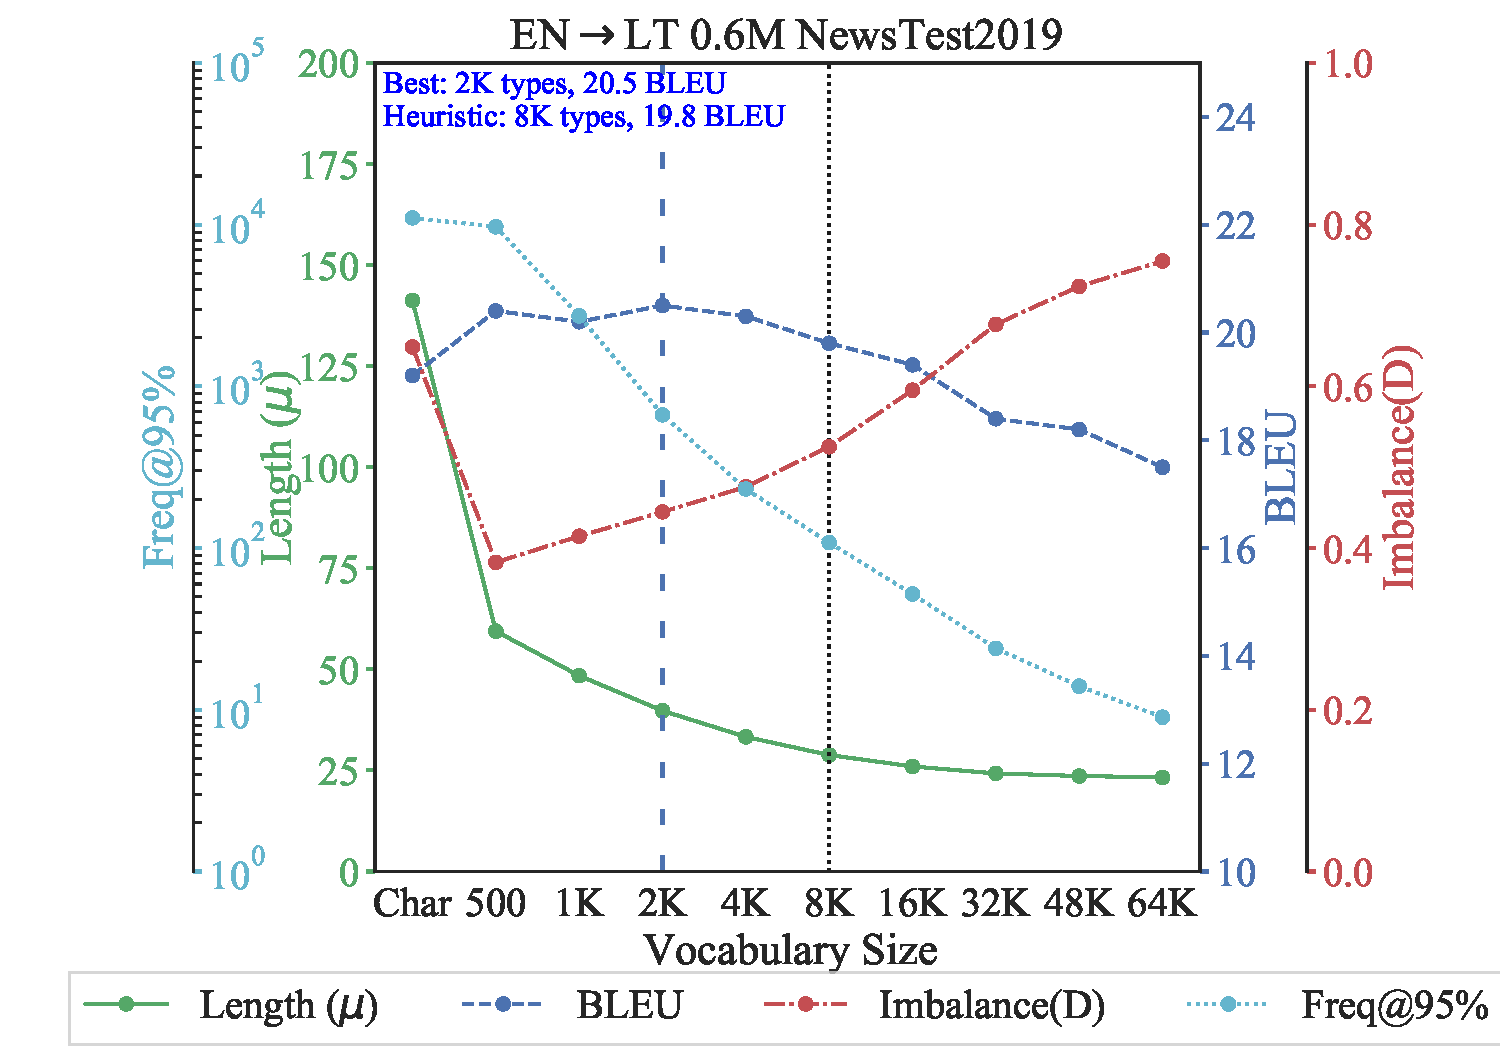
\includegraphics[width=0.96\linewidth,trim={2.4cm 1.32cm 1.4cm 0},clip]{4axv-test-enlt-0.6m.pdf}
  %\caption{1c}
  %\label{fig:sfig2}
\end{subfigure}


\caption{Visualization of sequence length ($\mu$) (lower is better), class imbalance (D) (lower is better), frequency of $95^{th}$ percentile class ($\mathcal{F}_{95\%}$) (higher is better; plotted in logarithmic scale), and test set BLEU (higher is better) on all language pairs and training data sizes. % Visualizations on validation sets is provided in Appendix~\ref{sec:appendix}.
The vocabulary sizes that achieved highest BLEU are indicated with dashed vertical lines, and the vocabulary our heuristic selects is indicated by dotted vertical lines.}
\label{fig:mu-d-freq-bleu-part2}
\end{figure}


BLEU scores for DE$\rightarrow$EN and EN$\rightarrow$DE experiments are reported in Figures~\ref{fig:bleu-deen} and \ref{fig:bleu-ende} respectively.
Results from EN$\rightarrow$HI, and EN$\rightarrow$LT are combined in Figure~\ref{fig:bleu-enhilt}. %\footnote{The SOTA results for these test sets can be found at \url{http://matrix.statmt.org} for EN$\leftrightarrow$DE and EN$\rightarrow$LT, and at \url{http://lotus.kuee.kyoto-u.ac.jp/WAT/evaluation/list.php?t=13&o=7} for EN$\rightarrow$HI. Often the SOTA results relies on more resources than Table~\ref{tab:datasets}.}
All the reported BLEU scores are obtained using \textsc{SacreBLEU} \cite{post-2018-sacreBLEU}.\footnote{\texttt{BLEU+case.mixed+numrefs.1+smooth.exp+tok.13a+version.1.4.6}}

We make the following observations: smaller vocabulary such as characters have not produced the best BLEU for any of our language pairs or dataset sizes.
A vocabulary of 32K or larger is unlikely to produce optimal results unless the data set is large e.g. the 4.5M DE$\leftrightarrow$EN sets.
The BLEU curves as a function of vocabulary sizes have a shape resembling a hill.
The position of the peak of the hill seems to shift towards a larger vocabulary when the datasets are large.
However, there is a lot of variance in the position of the peak: one extreme is at 500 types on 0.5M EN$\rightarrow$HI, and the other extreme is at 64K types in 4.5M DE$\rightarrow$EN. %\footnote{or possibly beyond 64K, but search on such larger vocabularies is beyond the scope of this work as it requires more computational resources.}

Although Figures~\ref{fig:bleu-ende-deen} and \ref{fig:bleu-enhilt} indicate \textit{where} the optimal vocabulary size is for these chosen language pairs and datasets, the question of \textit{why} the peak is where it is remains unanswered.
We visualize $\mu$, $D$, and $F_{95\%}$ in Figures~\ref{fig:mu-d-freq-bleu-part1} and \ref{fig:mu-d-freq-bleu-part2} to answer that question, and report these observations:
\begin{enumerate}
    \itemsep0em
    %\item Using a larger vocabulary of 32K and above is harmful on small and medium datasets. A minimal vocabulary containing only characters also did not produce a best BLEU in any setting.
    \item Small vocabularies have a relatively larger $\mathcal{F}_{95\%}$ (favorable to classifier), yet they are sub-optimal. We reason that this is due to the presence of a larger $\mu$, which is unfavorable to the autoregressor.
    \item Larger vocabularies such as 32K and beyond have a smaller $\mu$ which favors the autoregressor, yet rarely achieved the best BLEU.
    We reason this is due to the presence of a lower $\mathcal{F}_{95\%}$ and a higher $D$ being unfavorable to the classifier.
    Since the larger datasets have many training examples for each class, as indicated by a generally larger $\mathcal{F}_{95\%}$, we conclude that bigger vocabularies tend to yield optimal results compared to smaller datasets in the same language.

    \item On small (30K) to medium (1.3M) data sizes, the vocabulary size of 8K seems to find a good trade-off between $\mu$ and $D$, as well as between $\mu$ and $\mathcal{F}_{95\%}$.%, and hence serves as a safer choice tha.
\end{enumerate}

 There is a \textit{simple heuristic} to locate the peak: the near-optimal vocabulary size is where sentence length $\mu$ is small, while $\mathcal{F}_{95\%}$ is approximately $100$ or higher.
BLEU scores are often lower at larger vocabulary sizes---where $\mu$ is (favorably) low but $D$ is (unfavorably) high (Figures~\ref{fig:mu-d-freq-bleu-part1} and \ref{fig:mu-d-freq-bleu-part2}).
This calls for a further investigation that is reported in the following section.

%%%%%%%%%%%%%%%%%%%%%%%%%%%%%%%%%%%%%%%%%%
\section{Evaluating MT as Classification}
\label{sec:mt-eval-as-cls}

Section \ref{sec:classifier-nlg} provides a high-level view of NMT as two fundamental ML components: an autoregressor and a classifier. 
Specifically, NMT is viewed as a multi-class classifier that operates on representations from an autoregressor.
We may thus consider the well known evaluation metrics such as precision, recall, and F-measure.

Consider a test corpus, $T = \{ (x^{(i)}, h^{(i)}, y^{(i)}) | i = 1,2,3...m \}$ where $x^{(i)}$, $h^{(i)}$, and $y^{(i)}$ are source, system hypothesis, and reference translation, respectively. Let $x = \{x^{(i)} \forall i\}$ and similar for $h$ and $y$.  Let $V_h, V_y, V_{h\cap y},$ and $V$ be the vocabulary of $h$, the vocabulary of $y$, $V_h \cap V_y$, and $V_h \cup V_y$, respectively.
%As multiple-references in MT evaluation are increasing rare nowadays, and for simplicity, we limit our scope to single-reference only.
%We treat each word type in vocabulary $V$ as a class in a multi-class classifier.
For each class $c \in V$, 
\begin{align*}
 \textsc{Preds}(c) &= \sum_{i=1}^m C(c, h^{(i)}) ; \hspace*{1.5cm} \textsc{Refs}(c) = \sum_{i=1}^m C(c, y^{(i)})\\
\textsc{Match}(c) &= \sum_{i=1}^m min\{C(c, h^{(i)}), C(c, y^{(i)})\} 
\end{align*}
\noindent where $C(c, a)$  counts the number of tokens of type $c$ in sequence $a$, similar to \citet{papineni-etal-2002-bleu}. 
% and $k$ is a smoothing factor.\footnote{we use $k=1$}
For each class $c \in V_{h \cap y}$, precision ($P_c$), recall ($R_c$), and $F_\beta$ measure ($F_{\beta;c}$) are computed as follows:\footnote{We consider $F_{\beta;c}$ for $c \not\in V_{h \cap y}$ to be 0.}
\begin{align*}
    P_c &= \frac{\textsc{Match}(c)}{\textsc{Preds}(c)} \\
    R_c &= \frac{\textsc{Match}(c)}{\textsc{Refs}(c)} \\
    F_{\beta;c} &= (1 + \beta^2)  \frac{ P_c \times R_c}{ \beta^2 \times P_c + R_c}
\end{align*}

The overall performance of a multi-classifier is obtained by averaging individual class performances. The two most popular averaging methods are: \textit{macro-average}, which assigns equal importance to each type, and \textit{micro-average}, which assigns equal importance to each token, as follows:  
\begin{align*}
\maf\beta &= \frac{\sum_{c \in V} F_{\beta;c}} {|V|}\\
\mif\beta &= \frac{\sum_{c\in V} f(c) \times F_{\beta;c}} {\sum_{c'\in V} f(c')}
\end{align*}
\noindent where $f(c) = \textsc{Refs}(c)+k$ for smoothing factor $k > 0$.\footnote{We use $k=1$. If $k\rightarrow \infty$, then \mif1 $\rightarrow$ \maf1.} We scale $\maf\beta$ and $\mif\beta$ values to percentile, similar to \bleu, for the sake of easier readability.  Figure \ref{fig:bleu-damage} provides a visualization of \maf1 and \mif1 as well as the popular alternatives such as \bleu\ and \chrf1 in context.
%See Figure~\ref{fig:bleu-damage} for visual difference between \maf\beta and \mif\beta.
\begin{figure}[ht]
  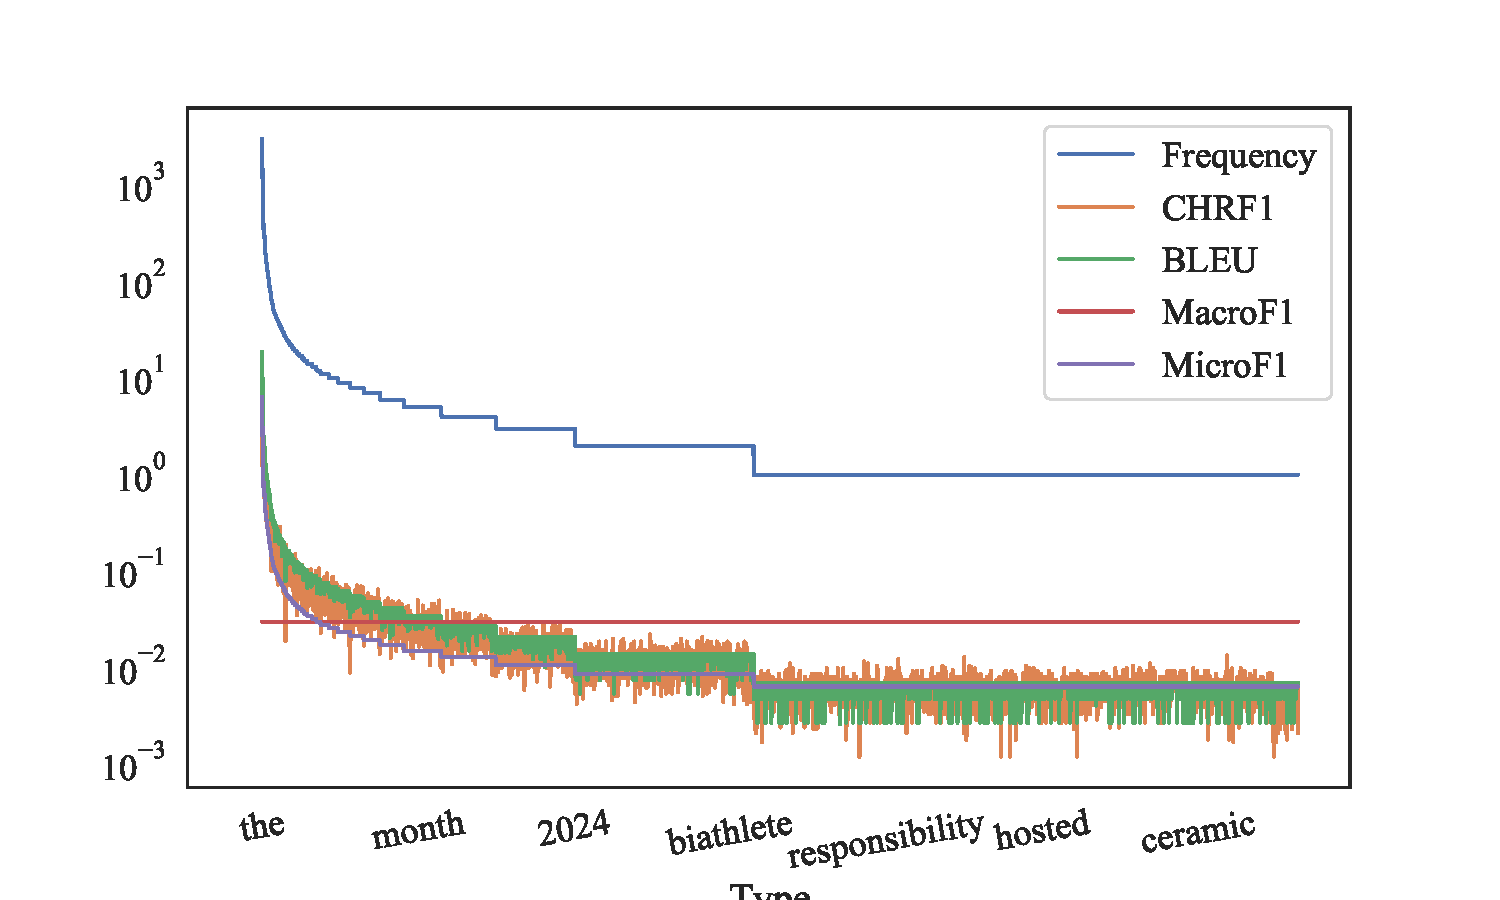
\includegraphics[width=0.75\linewidth,trim={15mm 5mm 25mm 15mm},clip]{img/bleu-chrf-macro-micro-swapin-lenmatch.pdf}
  \caption{MT metrics and their weight distribution across vocabulary as measured on WMT NewsTest2019 De-En corpus.
    The horizontal axis contains word types ranked by frequencies.
     The vertical axis, in logarithmic scale, represents type frequencies (raw count) and percentile of contribution to the total corpus-level score. 
     %The contribution of a type is defined as the difference in corpus-level score between when the type is perfectly learned versus when it is fully ignored~(i.e zero-recall). 
    %Perfect translations are simply when reference is treated as hypothesis where are as the full-ignorance or zero-recall is simulated for each type by replacing an out-of-vocabulary token of similar character count in the perfectly translated hypothesis~(therefore, no effect on length penalty).
    The weight of a type is the loss in corpus-level MT score when each token of the type is replaced by an out-of-vocabulary token of similar character count.
     The roughness in \bleu\ and \chrf1 lines is due to the variation in n-grams affected by a type.
     \mif1 uses only unigrams and scales the contribution by its frequency, whereas
     \maf1 is unweighted and assigns equal importance to all the types regardless of their frequencies. 
   It is evident that the type contribution in \bleu\ and \chrf1 is scaled according to frequencies in the similar manner as \mif1.
    For instance, `the' type appears 3019 times in the chosen test corpus, and zero-recall of `the' results in a loss up to 18.83\%, 9.38\%, 6.45\%, and 0.03\% of overall score in \bleu, \chrf1, \mif1, and \maf1, respectively.}
  %\Description{???.}
  \label{fig:bleu-damage}
\end{figure}



%%%%%%%%%%%%%%%%%%%%%%%%%%%%%%%%%%%%%%%%%%%%%%%%%%%%%%%%%%%%%%%%%%%%%%%%%%%%
\section{Measuring Classifier Bias Due to Imbalance}
\label{sec:class-bias}

In a typical classification setting with imbalanced classes, the classifier learns an undesired bias based on frequencies.
%Specifically, a biased classifier overclassifies frequent classes, leading to over recall but poor precision of frequent words, and underclassifies rare classes, leading to poor recall of rare words.
A balanced class distribution debiases in this regard, leading to improvement in the precision of frequent classes as well as recall of infrequent classes.
However, BLEU focuses only on the \textit{precision} of classes; except for adding a global brevity penalty, it is ignorant of the poor recall of infrequent classes.
%\footnote{There is a plenty of criticism on BLEU in the literature already \cite{ccb-2007-metaeval}.}
Therefore, the BLEU scores shown in Figures~\ref{fig:bleu-deen}, \ref{fig:bleu-ende} and \ref{fig:bleu-enhilt} capture only a part of the improvements and biases.
In this section we perform a detailed analysis of the impact of class balancing by considering both precision \textit{and} recall of classes.
%\footnote{The original reason BLEU was defined as a precision-only measure in the intent to use multiple references. This is exceedingly rare nowadays, so we are inclined toward advocating F-1 as an acceptable measure.}

We accomplish this in two stages:
First, we define a method to measure the bias of the model for classes based on their frequencies.
Second, we track the bias in relation to vocabulary size and class imbalance, and report DE$\rightarrow$EN and EN$\rightarrow$DE, as these have many data points.

\subsection{Frequency Based Bias}
We measure frequency bias using the Pearson correlation coefficient, $\rho$, between class rank and class performance, where for performance measures we use precision and recall.
Classes are ranked based on descending order of frequencies in the \textit{training data} encoded with the same encoding schemes used for reported NMT experiments.
With this setup, the class with rank 1, say $\mathcal{R}_1$, is the one with the highest frequency, rank 2 is the next highest, and so on.
More generally, $\mathcal{R}_k$ is an index in the class rank list which has an inverse relation to class frequencies.


The Pearson correlation coefficients between class rank and precision ($\rho_{\mathcal{R}, P}$), and class rank and recall ($\rho_{\mathcal{R}, R})$ are reported in Figure \ref{fig:corr-deen-test}.
In datasets where $D$ is high, the performance of classifier correlates with class rank. Such correlations are undesired for a classifier.

\begin{figure}[ht]
\begin{subfigure}{0.495\linewidth}
    \centering
    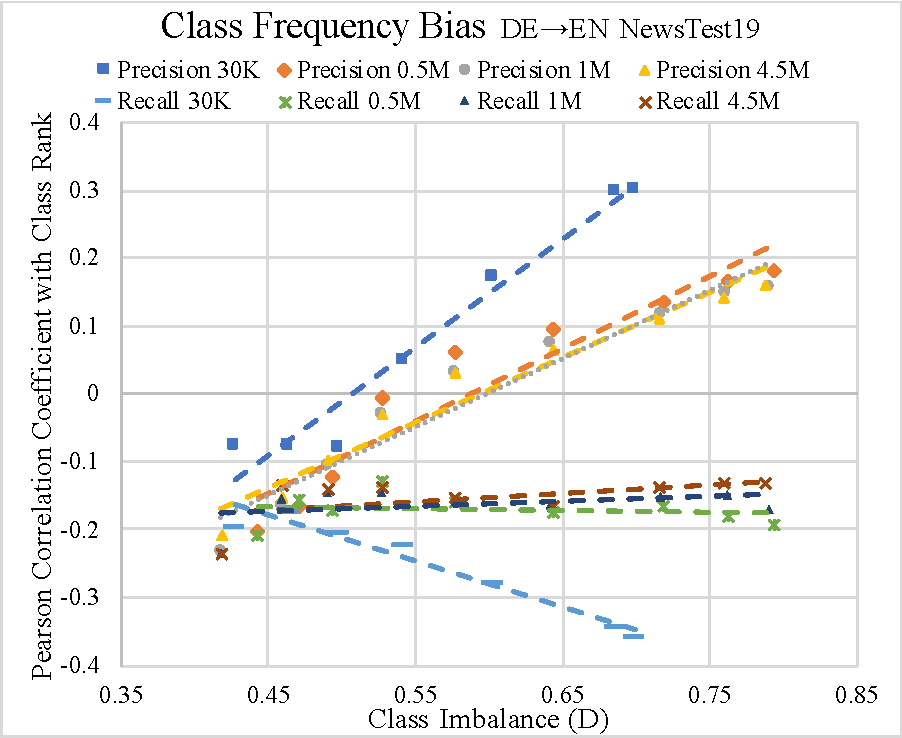
\includegraphics[width=\linewidth]{corr-deen-test.pdf}
\end{subfigure}
\begin{subfigure}{0.495\linewidth}
    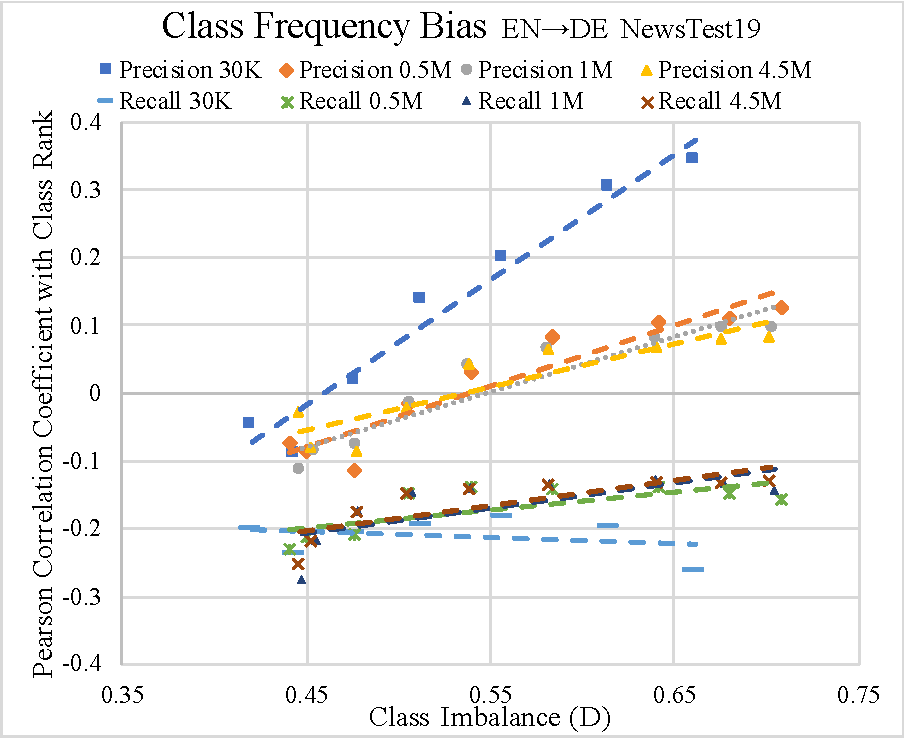
\includegraphics[width=\textwidth,clip]{corr-ende-test.pdf}
\end{subfigure}
        \caption{Correlation analysis on DE$\rightarrow$EN and EN$\rightarrow$DE show that NMT models suffer from frequency based class bias, indicated by non-zero correlation of both precision and recall with class rank.
        Reduction in class imbalance (D), as shown by the horizontal axis, generally reduces the bias as indicated by the reduction in magnitude of correlation.}
         \label{fig:corr-deen-test}
\end{figure}


%Figure \ref{fig:corr-enhi-enlt-test} contains visualization of frequency bias on EN$\rightarrow$DE and EN$\rightarrow$HI test sets.
%\begin{figure}[ht]
%\begin{subfigure}{0.495\linewidth}
%  \centering
%  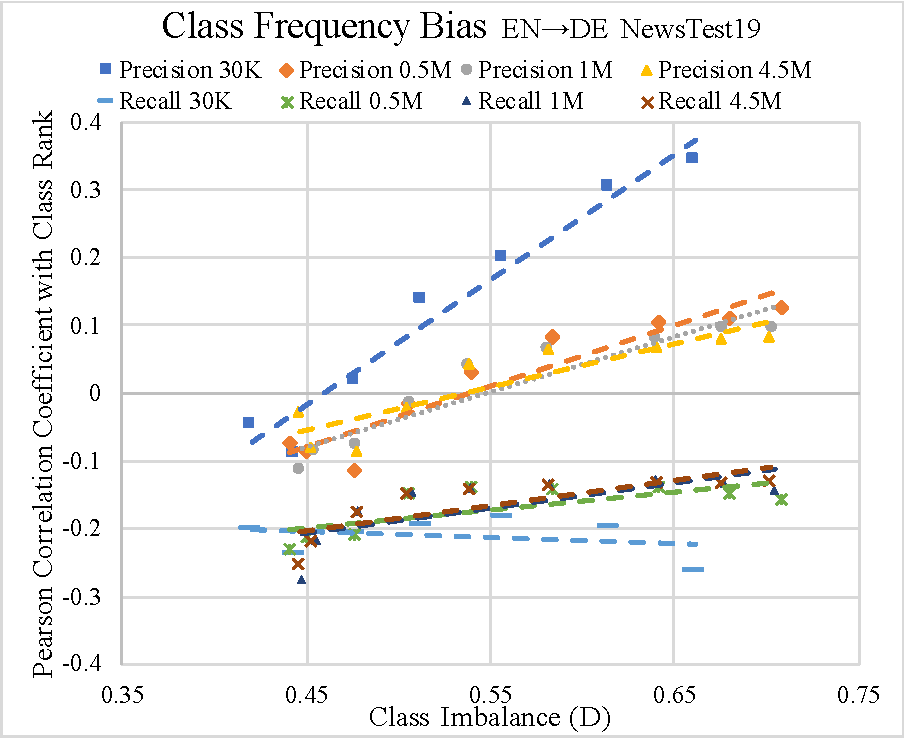
\includegraphics[width=\textwidth,clip]{corr-ende-test.pdf}
  %\caption{Correlation analysis on EN$\rightarrow$DE test set.}
%\end{subfigure}
%\begin{subfigure}{0.495\linewidth}
%  \centering
%  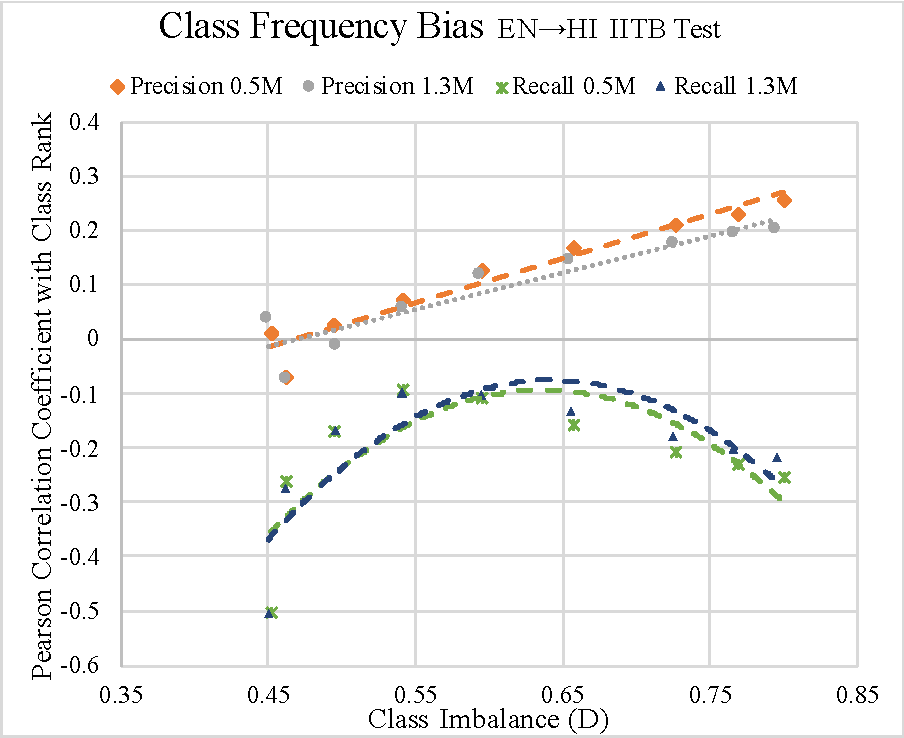
\includegraphics[width=\textwidth,clip]{corr-enhi-test.pdf}
  %\caption{Correlation analysis on EN$\rightarrow$HI test set.}
  %\label{fig:sfig1}
%\end{subfigure}
%\caption{Correlation analysis on EN$\rightarrow$DE, and EN$\rightarrow$HI test sets. The non-zero correlation of precision and recall with class rank indicate the class frequency bias in NMT models.}
%\label{fig:corr-enhi-enlt-test}
%\end{figure}


\subsection{Analysis of Class Frequency Bias}
An ideal classifier is one that does not discriminate classes based on their frequencies, i.e. one that exhibits no correlation between $\rho_{\mathcal{R}, P}$, and $\mathbf{r}_{\mathcal{R}, R}$.
However, we see in Figure~\ref{fig:corr-deen-test} that:
\begin{enumerate}
    \itemsep0em
    \item $\rho_{\mathcal{R}, P}$ is positive when the dataset has high $D$; i.e if the class rank increases (frequency decreases), precision increases in relation to it.
    This indicates that frequent classes have relatively less precision than infrequent classes.
    The bias is strongly positive on smaller datasets such as 30K DE$\rightarrow$EN, which gradually diminishes if the training data size is increased or a vocabulary setting is chosen to reduce $D$.
    \item $\rho_{\mathcal{R}, R}$ is negative, i.e., if the class rank increases, recall decreases in relation to it.
    This is an indication that infrequent classes have relatively lower recall than frequent classes.
\end{enumerate}
Figure~\ref{fig:corr-deen-test} shows a trend that frequency based bias measured by correlation coefficient is lower in settings that have lower $D$.
However, since $D$ is non-zero, there still exists non-zero correlation between recall and class rank ($\rho_{\mathcal{R}, R}$), indicating the poorer recall of low-frequency classes.
%This analysis does not consider the indirect effect of $\mu$

% \ref{sennrich-etal-2016-bpe}, with manual analysis, reported that BPE not only solved and improved translation of OOV words, it also improved the translation of certain in-vocabulary words. We note this behaviour due to an increased precision of frequent classes after class balancing.


%%%%%%%%%%%%%%%%%%%%%%%%%%%%%%%%%%%%%%%%%%%%%%%%%%%%%%%%%%%%%%%%%%%%%%%%%%%%
\section{Justification for Evaluating MT as Classifier}
\label{sec:justific-mt-eval}

In the following sections, we verify and justify the utility of \maf1 while also offering a comparison with popular alternatives such as \mif1, \bleu~\cite{papineni-etal-2002-bleu}, \chrf{1}~\cite{popovic-2015-chrf}, BLEURT~\cite{sellam-etal-2020-bleurt}. \bleu\ and \chrf1 scores are computed using \textsc{SacreBleu}~\cite{post-2018-sacreBLEU}. %and has signature \texttt{\small BLEU+case.mixed+lang.<xx>-<yy>+numrefs.1 +smooth.exp+tok.<TOK>+version.1.4.13}, where \texttt{<TOK>} is \texttt{zh} for Chinese, and \texttt{13a} for all other languages. 
\maf1 and \mif1 use the same tokenizer as \bleu.
%\chrf1 is also obtained using \textsc{SacreBleu} and has signature \texttt{\small chrF1+lang.<xx>-<yy>+numchars.6+space.false +version.1.4.13}
 Since BLEURT is a segment-level measure, we consider both \blrtmn\ and \blrtmd, which are mean and median of segment-level scores, as its corpus-level measures. 
We use Kendall's rank correlation coefficient, $\tau$, to compute the association between metrics and human judgments.
%, as $\tau$ is robust to outliers than Pearson $r$ \cite{croux2010robust-correlation}. 
%The correlation values and their p-values are computed using \texttt{scipy.stats} package \cite{2020SciPy-NMeth}. 
Correlations with p-values smaller than $\alpha=0.05$ are considered to be statistically significant.


\subsection{Data-to-Text: WebNLG}
\label{sec:webnlg}


\begin{table}[ht]
    \footnotesize
    \centering
    \begin{tabular}{lrr}
%& \multicolumn{2}{c}{ Kendall $\tau$ }\\
Name & Fluency \& Grammar & Semantics \\ \hline\hline
\bleu\  & \insig.444 & \insig.500 \\
\chrf1 & \insig.278    & .778   \\
\maf1  & \insig.222    & .722   \\
\mif1  & \insig.333    & .611   \\ \hline
\blrtmn & \insig.444   & .833   \\
\blrtmd & .611  & .667   \\
\end{tabular}
    \caption{\small WebNLG data-to-text task: Kendall's $\tau$ between system-level MT metric scores and human judgments.
    Fluency and grammar are correlated identically by all metrics.
    Values that are \textit{not} significant at $\alpha=0.05$ are indicated by \insig{}.}
    \label{tab:webnlg-kendall}
\end{table}


We use the 2017 WebNLG Challenge dataset \cite{gardent2017webNLG-corpus, shimorina2018webnlg-human-eval}\footnote{\myurl{https://gitlab.com/webnlg/webnlg-human-evaluation}} to analyze the differences between micro- and macro- averaging. 
WebNLG is a task of generating English text for sets of triples extracted from DBPedia.
Human annotations are available for a sample of 223 records each from nine NLG systems.
%The quality of generated sentences is judged along three linguistic aspects: fluency, grammar, and semantics.\footnote{We treat semantics as semantic adequacy.}
The human judgments provided have three linguistic aspects---fluency, grammar, and semantics\footnote{Fluency and grammar, which are elicited with nearly identical directions \cite{gardent2017webNLG-corpus}, are identically correlated.}---which enable us to perform a fine grained analysis of our metrics.
We compute Kendall's $\tau$ between metrics and human judgments, which are reported in Table~\ref{tab:webnlg-kendall}.

As seen in Table~\ref{tab:webnlg-kendall}, the metrics exhibit much variance in agreements with human judgments. %Fluency and grammar display same correlations and hence are com  
For instance, \blrtmd\ is the best indicator of fluency and grammar, however \blrtmn\ is best on semantics. 
BLEURT, being a \textit{model-based} measure that is directly trained on human judgments, scores relatively higher than others.
Considering the model-free metrics, chrf1 does well on semantics but poorly on fluency and grammar compared to \bleu.
Not surprisingly, both \mif1 and \maf1, which rely solely on unigrams, are poor indicators of fluency and grammar compared to \bleu, however \maf1 is clearly a better indicator of semantics than \bleu. 
The discrepancy between \mif1 and \maf1 regarding their agreement with fluency, grammar, and semantics is expected: micro-averaging pays more attention to function words (as they are frequent types) that contribute to fluency and grammar whereas macro-averaging pays relatively more attention to the content words that contribute to semantic adequacy. 
%\mableu, by extending \maf1 with higher order n-grams, is found to have a good agreement with semantic adequacy while a better agreement in fluency and grammar than \maf1.

The take away from this analysis is as follows: \maf1 is a strong indicator of semantic adequacy, however, it is a poor indicator of fluency. We recommend using either \maf1 or \chrf1 when semantic adequacy and not fluency is a desired goal.
%Caveat: WebNLG is a small dataset, and English only. 
%In the next section, we use larger datasets from tens of languages.



\subsection{Machine Translation: WMT Metrics}
\label{sec:wmt-metrics}

\begin{table*}[ht!]
    %\footnotesize
    \small
    \centering
    
\begin{tabular}{r r l r r r r r }
Year & Pairs  & & $\star$\bleu\ & \bleu\ & \maf1 & \mif1 & \chrf1 \\ \hline\hline
\multirow{3}{*}{ 2019 } 
    & \multirow{3}{*}{18}
     & Mean   & .751 & .771 & .821 & .818 & .841  \\ 
   & & Median & .782 & .752 & .844 & .844 & .875  \\
   & & Wins   &     3 &     3 &  \textbf{6}    &     3 &   5 \\ \hline
  %& SD     & 0.124 & 0.101 & 0.112 & 0.093 & 0.095 \\ \\
\multirow{3}{*}{ 2018 } 
  & \multirow{3}{*}{14}
   & Mean   & .858 & .857 & .875 & .873 & .902  \\ 
  & & Median & .868 & .868 & .901 & .879 & .919  \\
  & & Wins    &  1  &  2 & 3 &  2 &  \textbf{6}\\ \hline  
  %& SD     & 0.077 & 0.080 & 0.087 & 0.062 & 0.052  \\ \hline  
\multirow{3}{*}{ 2017 }
   & \multirow{3}{*}{13}
    & Mean   & .752 & .713 & .714 & .742 & .804 \\  
  & & Median & .758 & .733 & .735 & .728 & .791 \\
  & & Wins   & 5 & 4 & 2 & 2 & \textbf{6} \\
  %& SD     & 0.132 & 0.110 & 0.103 & 0.097 & 0.088 & 0.099 & 0.093 & 0.099 \\  
\end{tabular}   
\caption{WMT 2017--19 Metrics task: Mean and median Kendall's $\tau$ between MT metrics and human judgments.
%Only the mean and median $\tau$, and number of wins are reported in this table.
Correlations that are not significant at $\alpha=0.05$ are excluded from the calculation of mean, and median, and wins.
%`Wins' is number of times the achieved highest agreement with human judgments, out of total pairs in `Pairs' column.
See Appendix Tables \ref{tab:wmt19-kendall}, \ref{tab:wmt18-kendall}, and \ref{tab:wmt17-kendall} for full details.
%\maf1 and \mif1 use the same tokenizer as \bleu, whereas $\star$\bleu\ is pre-computed scores available in WMT Metrics package.
$\star$\bleu\ is pre-computed scores available in the metrics packages.
In 2018 and 2019, both \maf1 and \mif1 outperform \bleu, \maf1 outperforms \mif1.
\chrf1 has strongest mean and median agreements across the years.
Judging based on the number of wins, \maf1 has steady progress over the years, and outperforms others in 2019.
%A few outliers (that were found to be result of poor quality references) are excluded from the calculation of mean and standard deviation.
}
\label{tab:wmt-summary}
\end{table*}

In this section, we verify how well the metrics agree with human judgments using Workshop on Machine Translation (WMT) metrics task datasets for 2017--2019~\cite{WMT17-metrics,WMT18-metrics,WMT19-metrics-proceedings}.\footnote{\myurl{http://www.statmt.org/wmt19/metrics-task.html}}
%These datasets contain multiple translation directions (i.e. source$\rightarrow$target languages), and each direction contains outputs from multiple MT models along with their human judgments. 
%Unlike WebNLG, here the human judgments are a single score.
We first compute scores from each MT metric, and then calculate the correlation $\tau$ with human judgments.

As there are many language pairs and translation directions in each year, we report only the mean and median of $\tau$, and number of wins per metric for each year in Table \ref{tab:wmt-summary}. %\footnote{We report $\tau$ for individual translation directions in Tables \ref{tab:wmt19-kendall}, \ref{tab:wmt18-kendall}, and \ref{tab:wmt17-kendall} of Appendix.}
We have excluded BLEURT from comparison in this section since the BLEURT models are fine-tuned on the same datasets on which we are evaluating the other methods.\footnote{\myurl{https://github.com/google-research/bleurt}}
\chrf1 has the strongest mean and median agreement with human judgments across the years.
In 2018 and 2019, both \maf1 and \mif1 mean and median agreements outperform \bleu\, whereas in 2017 \bleu\ was better than \maf1 and \mif1.%, however \chrf1 has the strongest agreements with human judgments across the years.

%We observe that the polarity of difference between mean \maf1 and mean \mif1 has changed over the years: i.e. human agreements were better with \mif1 than \maf1 in 2017, whereas in 2019, human judgments agree better with \maf1 than \mif1.
%We observe in the recent years of WMT that \chrf1 and \maf1 outperform \bleu.
%This observation is interesting for the same reason as \maf1 outperforming \mif1.
As seen in Section~\ref{sec:webnlg}, \maf1 weighs towards semantics whereas \mif1 and \bleu\ weigh towards fluency and grammar.
This indicates that recent MT systems are mostly fluent, and adequacy is the key discriminating factor amongst them.
\bleu\ served well in the early era of statistical MT when fluency was a harder objective. 
Recent advancements in neural MT models such as Transformers \cite{vaswani2017attention} produce fluent outputs, and have brought us to an era where semantic adequacy is the focus.


% save it for the slides
%We envision that the methods such as \maf1 that emphasize the long tail be more successful in the future years, and this vision is inline with \citet{steedman-2008-last}:
%One day, either because of the demise of Moore’slaw, or simply because we have done all the easy stuff, the Long Tail will come back to haunt us.
%\textit{``One day, ... simply because we have done all the easy stuff, the Long Tail will come back to haunt us.''}


\subsection{Cross-Lingual Information Retrieval}
\label{sec:clir}
In this section, we determine correlation between MT metrics and  downstream cross-lingual information retrieval (CLIR) tasks.
CLIR is a kind of information retrieval (IR) task in which documents in one language are retrieved given queries in another~\cite{grefenstette2012CLIR}. 
A practical solution to CLIR is to translate source documents into the query language using an MT model, then use a monolingual IR system to match queries with translated documents. 
Correlation between MT and IR metrics is accomplished in the following steps: 
\begin{enumerate}[noitemsep,topsep=0pt]
 \item Build a set of MT models and measure their performance using MT metrics.
 \item Using each MT model in the set, translate all source documents to the target language, build an IR model, and measure IR performance on translated documents.
 \item For each MT metric, find the correlation between the set of MT scores and their corresponding set of IR scores.
 The MT metric that has a stronger correlation with the IR metric(s) is more useful than the ones with weaker correlations.
\item Repeat the above steps on many languages to verify the generalizability of findings.
\end{enumerate}

%\begin{figure}[ht]
%\centering
%\includegraphics[width=0.9\linewidth,trim={0cm 0 0cm 0},clip]{img/CLIR-Pipe.pdf}
% to modify, goto https://docs.google.com/drawings/d/1ZrukLOtH3fQPyl9SkLWqrUqsbrSofDlSXC1tFwpYs2E/edit 
%\caption{Cross-lingual Information Retrieval system}
%\label{fig:clir-pipe}
%\end{figure}

An essential resource of this analysis is a dataset with human annotations for computing MT and IR performances.
%Specifically, this analysis requires datasets that have documents in source language and queries in target language,  along with the human translation of documents to calculate scores from MT measures, and human judgments of query to document relation to calculate IR performance.
%In addition, such datasets for a diverse set of languages are desired to verify the generalizabilty of findings.
%IARPA's Machine Translation for English Retrieval of Information in Any Language (MATERIAL) program\footnote{\myurl{https://www.iarpa.gov/index.php/research-programs/material/material-baa}} and made such datasets available, however only to its participants. 
%We conduct experiments on data from the 2020 workshop on \textit{Cross-Language Search and Summarization of Text and Speech} (CLSSTS) \cite{zavorin-etal-2020-corpora}.
%he restricted-access MATERIAL datasets using the systems submitted by MATERIAL performers where high-quality human judgments are available, and secondly, on publicly available datasets prepared by with a few assumptions on query-relevance judgments.

%\subsubsection{CLSSTS Datasets}
%\label{sec:material}

\begin{table*}[ht]
    \footnotesize
    \begin{tabular}{l l l r r r r r r }
 & Domain & IR Score & \bleu\ & \maf1 & \mif1 & \chrf1 & \blrtmn & \blrtmd \\\hline\hline

\multirow{4}{*}{LT-EN} 
& \multirow{2}{*}{In} 
  & AQWV & .429 & \insig.363 & \textbf{.508} & \insig.385 & .451  & .420 \\
& & MAP  & .495  & .429      & \textbf{.575} & .451       & .473  & .486 \\
& \multirow{2}{*}{In+Ext}
   & AQWV & \insig.345 & \textbf{.527} & .491  & .491 & .491 & .477 \\
&  & MAP  & \insig.273 & \insig\textbf{.455} & \insig.418 & \insig.418 & \insig.418 & \insig.404 \\\hline
\multirow{4}{*}{PS-EN}
  & \multirow{2}{*}{In} 
    & AQWV  & .559 & \textbf{.653} & .574 & .581 & .584 & .581  \\
  & & MAP   & .493 & \textbf{.632} & .487 & .494 & .558 & .554 \\
  & \multirow{2}{*}{In+Ext}
    & AQWV   & .589 & \textbf{.682} & .593 & .583 & .581 & .571 \\
  & & MAP    & .519 & \textbf{.637} & .523 & .482 & .536 & .526 \\\hline
\multirow{4}{*}{BG-EN}
 & \multirow{2}{*}{In} 
    & AQWV   & \insig.455 & \textbf{.550}   & .527  & \insig.382 & \insig.418  & .418 \\ 
 &  & MAP    &  .491      &  \textbf{.661}  & .564  &  .491       & .527       & .527 \\ 
 & \multirow{2}{*}{In+ext}
    & AQWV   & \insig.257 & \textbf{.500}       & \insig.330 & \insig.404 & \insig.367 & \insig.367 \\
 &  & MAP   & \insig.183 & \insig\textbf{.426} & \insig.257 & \insig.330 & \insig.294 & \insig.294 
\end{tabular} 
\caption{CLSSTS CLIR task: Kendall's $\tau$ between IR and MT metrics under study.
The rows with Domain=In are where MT and IR scores are computed on the same set of documents, whereas Domain=In+Ext are where IR scores are computed on a larger set of documents that is a superset of segments on which MT scores are computed.
\textbf{Bold} values are the best correlations achieved in a row-wise setting; values with \insig~ are \textit{not} significant at $\alpha=0.05$.}
\label{tab:material-kendall}
\end{table*}

An essential resource of this analysis is a dataset with human annotations for computing MT and IR performances.
We conduct experiments on data from the 2020 workshop on \textit{Cross-Language Search and Summarization of Text and Speech} (CLSSTS) \cite{zavorin-etal-2020-corpora}.
CLSSTS datasets contain queries in English~(EN), and documents in many source languages along with their human translations, as well as query-document relevance judgments. 
We use three source languages: Lithuanian~(LT), Pashto~(PS), and Bulgarian~(BG).
The performance of this CLIR task is evaluated using two IR measures: Actual Query Weighted Value (AQWV) and Mean Average Precision (MAP).
AQWV\footnote{\href{https://www.nist.gov/system/files/documents/2017/10/26/aqwv\_derivation.pdf}{https://www.nist.gov/system/files/documents-/2017/10/26/aqwv\_derivation.pdf}} is derived from Actual Term Weighted Value (ATWV) metric \cite{wegmann2013ATWV}. 
%, being the official metric of MATERIAL program,
% by National Institute of Standards and Technology~(NIST). 
%The nature of AQWV is such that a higher score implies better CLIR performance. 
%Since the focus of this analysis is on MT evaluation methods and not the MT systems, we treat all MT systems as blackboxes for which internal details are unnecessary; however, we clarify that the MT systems used are representative of commonly used models such as convolutional \cite{gehring2017cnn} and Transformer~\cite{vaswani2017attention} NMT models, as well as once-popular syntax-based string-to-tree statistical MT~\cite{galley-etal-2004-sbmt}.


%The high level overview of our CLIR pipeline is shown in Figure \ref{fig:clir-pipe}:
%First, documents in source language are translated to English using a set of MT models. 
%Performance of all MT models is evaluated on the same set of documents using their corresponding human translations.
%The translated documents are indexed by an IR system, and the end-to-end performance on a set of queries is evaluated using AQWV metric with the help of human created judgments.
Our CLIR system is based on \citet{boschee-etal-2019-saral}, which is competitive in the workshop on CLSSTS-2020~\cite{clssts-2020}.
Since the CLIR system is also treated as a blackbox, the internals of CLIR is unnecessary and beyond the scope of this work.
%We use a single CLIR system with the same IR settings for all MT models in the set,\footnote{Details of IR and MT models anonymized} and measure Kendall's $\tau$ between MT and IR measures.
Kendall's $\tau$ between MT and IR measures, given in Table~\ref{tab:material-kendall}, show that \maf1 is the strongest indicator of CLIR downstream task performance in five out of six settings.
AQWV and MAP have a similar trend in agreement to the MT metrics.
\chrf1 and BLEURT, which are strong contenders when generated text is directly evaluated by humans, do not indicate CLIR task performance as well as \maf1, as CLIR tasks require faithful meaning equivalence across the language boundary, and human translators can mistake fluent output for proper translations \cite{callison-burch-etal-2007-meta}. 
%Hence, we recommend the use of \maf1 when MT output is used in downstream tasks such as IR.


